%-------------------------------------------------------------------------------
% This file provides a skeleton ATLAS document
%-------------------------------------------------------------------------------
% Specify where ATLAS LaTeX style files can be found
\newcommand*{\ATLASLATEXPATH}{latex/}
% Use this variant if the files are in a central location, e.g. $HOME/texmf
% \newcommand*{\ATLASLATEXPATH}{}
%-------------------------------------------------------------------------------
\documentclass[UKenglish,texlive=2013]{\ATLASLATEXPATH atlasdoc}
% The language of the document must be set: usually UKenglish or USenglish
% british and american also work!
% Selected options:
%  texlive=YYYY          Specify TeX Live version (2013 is default)
%  atlasstyle=true|false Use ATLAS style for document (default)
%  coverpage             Create ATLAS draft cover page for collaboration circulation
%                        See atlas-draft-cover.tex for a list of variables that should be defined.
%  cernpreprint          Create front page for a CERN preprint
%                        See atlas-preprint-cover.tex for a list of variables that should be defined.
%  PAPER                 The document is an ATLAS paper (draft)
%  CONF                  The document is a CONF note (only useful together with coverpage)
%  PUB                   The document is a PUB note (only useful together with coverpage)
%  txfonts=true|false    Use txfonts rather than the default newtx - needed for arXiv submission
%  paper=a4|letter       Set paper size to A4 (default) or letter
%  maketitle=true|false  Run or do not run \maketitle from the class

%-------------------------------------------------------------------------------
% Extra packages:
\usepackage{\ATLASLATEXPATH atlaspackage}
% Selected options:
%  biblatex=true|false   Use biblatex (default) or bibtex for the bibliography
%  backend=biber         Use the biber backend rather than bibtex
%  minimal               Minimal set of packages
%  default               Standard set of packages
%  full                  Full set of packages
% Style file with biblatex options for ATLAS documents
\usepackage{lineno}
\linenumbers
\usepackage{\ATLASLATEXPATH atlasbiblatex}

% Package for creating list of authors and contributors to the analysis
\usepackage{\ATLASLATEXPATH atlascontribute}

% Useful macros
\usepackage{\ATLASLATEXPATH atlasphysics}
% See doc/atlas-physics.pdf for a list of the defined symbols
% Default options are 
%   true:  journal, misc, particle, unit, xref
%   false: BSM, hion, math, process, other, texmf
% See the package for details on the options

% Files with references for use with biblatex
% Note that biber gives an error if it finds empty bib files
\addbibresource{TopRelatedModel.bib}
\addbibresource{bibtex/bib/atlas-paper.bib}

% Paths for figures - do not forget the / at the end of the directory name
\graphicspath{{logos/}{figures/}}

% Add you own definitions here (file TopRelatedModel-defs.sty)
\usepackage{TopRelatedModel-defs}
\def\ares{\ensuremath{a_{\mathrm{res}}}}
\def\anonres{\ensuremath{a_{\mathrm{non\mbox{-}res}}}}
\def\mfmet{\ensuremath{m(f_{\mathrm{met}})}}
\def\mvmet{\ensuremath{m(v_{\mathrm{met}})}}
\def\vmet{\ensuremath{v_{\mathrm{met}}}}
\def\fmet{\ensuremath{f_{\mathrm{met}}}}

%-------------------------------------------------------------------------------
% Generic document information
%-------------------------------------------------------------------------------

% Author and title for the PDF file
\hypersetup{pdftitle={Dark Matter Forum Draft (Top related models)},pdfauthor={Romain Madar}}
% Title, abstract and document 
\input{TopRelatedModel-metadata}

%-------------------------------------------------------------------------------
% Content
%-------------------------------------------------------------------------------
\begin{document}

\maketitle

\tableofcontents

% List of contributors - print here or after the Bibliography
%\AtlasPrintContribute{0.3}
\clearpage

%-------------------------------------------------------------------------------
\section{Motivations and models description}
\label{sec:MotivModelDescription}
%-------------------------------------------------------------------------------

In this note, we describe the phenomenology of dark matter models involving a strong coupling to the top quark.
These models can be classified according to their experimental signatures. Assuming the Standard Model (SM) flavour scheme, 
the models essentially lead to $\ttbar + \met$ final state and are described in a separated document. Since we do not know the flavour structure
of the dark sector, it is also interesting to relax this constraint and consider a different experimental signatures: monotop final state ($t+\met$)
and a prompt production of two top quarks having the same electric charge ($tt$)\footnote{For simplicity, the notation $tt$ is used to describe both $tt$ 
and $\bar{t}\bar{t}$}. These two final states are forbidden at the leading order in the SM
and become thus a good area to search for any new physics, and in particular dark matter.

\subsection{Model structure}

As usual, a dark matter candidate $\chi$ and a mediator $M$ (vectorial or scalar) need to be added to the SM to describe the dark sector and its
interaction with the SM particles. The full details of the various models are described in~\cite{AndreaFuksMaltoni,Agram:2013wda,,Cacciapagliaetal}, the basic ingredients are the following:
\begin{enumerate}
 \item the theory is effective and respects the $\SUtwoUone$ symmetry,
 \item the mediator strongly couples to the top quark,
 \item the top quark is \textit{singly} produced in association with a new particle $\Xnew$ (dark matter or mediator).
\end{enumerate}

There are two classes of models based on the monotop production mode: resonant and non-resonant production, as shown
in Fig.~\ref{fig:feyn_prod}. The sections~\ref{sec:ResonantProd} and~\ref{sec:NonResonantProd} describe the phenomenology leading to such production mechanisms.
Depending on the nature of $\Xnew$, two main final states might be relevant: monotop production or same-sign top quark pair production. 
Section~\ref{sec:ColliderSignature} discusses how the interplay of these two signatures can largely probe this class of dark matter model.

\begin{figure}[!h!tpd]
\centering
\includegraphics[width=0.31\textwidth]{feyn_diags/Resonant}
\includegraphics[width=0.31\textwidth]{feyn_diags/NonResonant}
\includegraphics[width=0.31\textwidth]{feyn_diags/NonResonant2}
%\subfigure[\label{subfig:S1}]{\includegraphics[width=0.46\textwidth]{feyn_diags/S1}}\\
%\subfigure[\label{subfig:S4_s}]{\includegraphics[width=0.46\textwidth]{feyn_diags/S4_s}}
%\subfigure[\label{subfig:S4_t}]{\includegraphics[width=0.46\textwidth]{feyn_diags/S4_t}}
\caption
{
%Feynman diagram of leading order processes leading to monotop events: production of
%a coloured scalar resonance $S$ decaying into a top quark and a spin-$1/2$ fermion $f_{met}$
%in the $\mathrm{S1_R}$ model~\subref{subfig:S1}, and $s$-\subref{subfig:S4_s}
%and $t$-\subref{subfig:S4_t} channel non resonant production of a top quark in association with
%a spin-1 boson $v_{met}$ in the $\mathrm{S4_R}$ model.
Feynman diagram of leading order processes leading to monotop events: resonant production of
$t$ via resonant mediator $M$ decaying into a top quark and $\Xnew$, which is the dark matter fermion $\chi$ (left),
and $s$ and $t$ channel non-resonant production of a top quark in association with $\Xnew$, which is the mediator $M$ (middle and right).
}
\label{fig:feyn_prod}

\end{figure}


\subsubsection{Resonant production}
\label{sec:ResonantProd}

In this case, the mediator $M$ is a couloured $2/3$-charged scalar $\phi^{\pm}$ decaying into a top quark and a spin-$1/2$ invisible particle, $\chi$ 
($\Xnew$ is then the dark matter candidate $\chi$). The dynamics of the new sector is then described by the following lagrangian:
\begin{equation}
 \label{eq:lagrangianResonant}
 \Lagr_{\mathrm{int}} \; = \; d^{C}_{i} \:  \left[ \left(g^{v}_{\phi d}\right)^{ij} +  \left(g^{a}_{\phi d}\right)^{ij} \gam^{5} \right] \: d_{j} \: \phi^{\pm} \; 
 + \; u^{C}_{k}  \left[ \left(g^{v}_{u\chi}\right)^{k} + \left(g^{a}_{u\chi}\right)^{k} \gam^{5} \right] \: \chi \: \phi^{\pm}
\end{equation}
where $u$ ($d$) stands for any $up$-quark ($down$-quark), the index $v$ ($a$) stands for vectorial (axial), $C$ means charge conjugate and $i,j,k$ run over the generations (color 
indices involved in the $\phi^{\pm}-$quarks interaction are not explicitly written).
The first term leads to the production of the mediator and the last term allows its decay into a $up$-quark 
and a non interacting fermion (in particular to the top quark when $\left(g^{v/a}_{u\chi}\right)^{k}$ is sizable mainly for $k=3$).
This model is then described by the masses of the mediator $m_{\phi}$ and the invisible fermion $m_{\chi}$, and the coupling 
$\left(g^{v/a}_{\phi d}\right)^{ij}$ and $\left(g^{v/a}_{u\chi}\right)^{k}$.

\com{Question/comment: in this resonant model, this is not so obvious to interpret $\phi_{\pm}$ as the mediator since there is a vertex $\phi-u-\chi$.
It is somehow breaking the concept of having a dark sector weakly coupled to ordinary matter via a mediator.}


\subsubsection{Non-resonant production}
\label{sec:NonResonantProd}

For the non-resonant production, the top quark is produced in association with the mediator 
($\Xnew$ is then the mediator and not the dark matter candidate). They are two possibilities 
depending on the nature of the mediator.

First, the mediator can be a scalar field interacting with the SM field and the dark matter candidate as described in this lagrangian:
\begin{equation}
 \label{eq:lagrangianNonResonantScalar}
 \Lagr_{\mathrm{int}} \; = \; u^{C}_{i} \:  \left[ \left(g^{v}_{\phi u}\right)^{ij} +  \left(g^{a}_{\phi u}\right)^{ij}  \gam^{5} \right] \: u_{j} \: \phi \; 
 + \; \chi^{C}  \left[ g^{v}_{\phi\chi} + g^{a}_{\phi\chi}  \gam^{5} \right] \chi \: \phi
\end{equation}
where $u$ stands for any $up$-quark, the index $v$ ($a$) stands for vectorial (axial), $C$ means charge conjugate and $i,j,k$ run over the generations.
The first term describes the interaction between the mediator and the $up$-quarks while the second term leads to the decay the mediator 
into invisible fermions. In this model, there is necessarily a mixing between $\phi$ and  the Higgs boson field. Additional parameters 
are then required to describe this new sector. Indeed, on top of the mediator mass and couplings, the mixing matrix of the two scalar fields
is needed in order to make predictions. For the sake of simplicity, we do not consider this case were the parameters 
space would be too large.

Another possibility is to consider a vectorial field as mediator with the following dynamics:
\begin{equation}
 \label{eq:lagrangianNonResonantVector}
  \Lagr_{\mathrm{int}} \; = \; \bar{u}_{i} \left[ \left(g^{v}_{Vu}\right)^{ij} \gam^{\mu} + \left(g^{a}_{Vu}\right)^{ij} \gam^{5} \right] u_{j} \: V_{\mu} \; 
  + \; \bar{\chi} \left[ g^{v}_{Vu} \gam^{\mu} + g^{a}_{V\chi} \gam^{5} \right]   \chi \: V_{\mu}
\end{equation}
where $u$ stands for any $up$-quark, the index $v$ ($a$) stands for vectorial (axial) and $i,j,k$ run over the generations.
The first term describes the interaction between the mediator and the $up$-quarks while the second term leads to the decay the mediator 
into invisible fermions. The new sector can be defined with the couplings $\left(g^{v/a}_{Vu}\right)^{ij}$, 
$g^{a/v}_{V\chi}$ and the masses $m_V$ and $m_{\chi}$. This model can be probed by two experimental signatures 
depending on the exact scenario: monotop and same-sign top quark production. 

\com{Question for theorists: why it cannot mix with $\Zboson$ in case of vectorial mediator ?}



\subsection{Simplifications}
 
The lagrangians from equations~\eqref{eq:lagrangianResonant} and~\eqref{eq:lagrangianNonResonantVector} contains too many degrees of freedom, 
which makes the LHC phenomenology difficult to predict. In addition, only a certain region of the parameter space can actually be probed with a monotop final state.
For these reasons, further simplifications are performed in particular in term of flavour and chiral structure of the model. 
These simplifications leads to some limitations in the way ATLAS and CMS can constrain the model parameter space and these limitations are also qualitatively discussed below.

\subsubsection{Flavour structure}

The flavour structure is simplified in order to have a reasonable signal production rate in proton-proton collisions.
In case of a scalar mediator, it has to be sufficiently produced so it has to couple with proton content, namely lightest quark which 
are allowed in equation~\eqref{eq:lagrangianResonant}. The monotop final state is sensitive to the scenario where $\phi$ strongly couples to $t\chi$.
\com{Correct and/or complete with the monotop paper}. In term of parameter space, it means that the monotop final state is not sensitive
to some parameters like coupling between the mediator and heavy quarks or the scenario in which $\BR{\phi}{t\chi} \ll 100 \%$. For the latest, 
there is a way to recover the sensitivity looking at $u_i d_j \to \phi \to u_i d_j$. Since $\phi$ must be produced, it has to coupled to quarks 
and must decay in the same final state. Experimentally, this would correspond to a di-jet resonance search.

The same kind of simplification is performed for the non-resonant production. The equation~\eqref{eq:lagrangianNonResonantVector} is simplified in the parameter
space where a monotop final state can be sufficiently produced to be detected at the LHC. The mediator $V$ must be produced from light quark initial state, 
in association with a top quark: this signature can mainly probe a high coupling $\left(g^{v/a}_{Vu}\right)^{13}_{Vu} \equiv g^{v/a}_{Vtu}$. Therefore,
the sensitivity to other flavour couplings is significantly lower since $V$ is less importantly produced. In addition, the mediator must decay into invisible particles
to lead to the searched monotop final state. As a consequence, the sensitivity for scenario where $\BR{V}{\chi\chi}\ll 100\%$ can be quite low. 
To cope with this second limitation, a same-sign top quark final state $gu \to tV(\to t\bar{u})$ is proposed to cover the cases where $V$ would decay
into visible particles. This case is more likely as the $tV$ production rate increases, and becomes then a key point to constraint this model in a consistent way.

\com{Questions for theorists:
\begin{itemize}
 \item How well these flavour assumptions are allowed by the other HEP data (proton decay life time, flavour physics, etc ...) ?
 \item MFV criteria ?
\end{itemize}
}

\subsubsection{Chiral structure}
\label{sec:chiralstructure}

The main point here is to consider only right handed quark components in order to not simplify the phenomenology. In fact, the representation of the left-handed 
components under the $\SUtwo$ symmetry imposes a coupling to $down$-type quarks, since the effective theory is invariant under $\SUtwoUone$ gauge symmetry. Having a coupling between
the mediator and $down$-type quarks fairly complicates the collider phenomenology in term of decay mode. Typically, including 
the left-handed components of quarks in the lagrangian~\eqref{eq:lagrangianNonResonantVector} describing the $Vtu$ vertex would lead to 
\begin{equation}
 \Lagr_{Vtu} \; = \;  g^{R}_{Vtu} \: \bar{t}_{R}\gam^{\mu}u_R \: V_{\mu} \; + \; g^{L}_{Vtu} \left(   \bar{t}_{L}\gam^{\mu}u_L \: + \:  \bar{b}_{L}\gam^{\mu}d_L \right) \: V_{\mu}
\end{equation}
where $g^{R/L} \equiv 1/2 \, (g^{v} \pm g^{a})$ couples only to right-handed/left-handed components. The second term ensure the invariance under $\SUtwo$ rotations, and lead to an additional decay mode $V \to b\bar{d} + \bar{b}d$ (on top of $V \to t\bar{u} + \bar{t}u$ and $V \to \chi\chi$). 
 
\subsection{Notations}

In section~\ref{sec:ColliderSignature}, the collider phenomenology and benchmark definition is discussed with notations which are 
a bit different\footnote{This difference is due to two things: the historical developpement on the monotop analysis and having a 
  common and simple set of notations for equations~\eqref{eq:lagrangianResonant},~\eqref{eq:lagrangianNonResonantScalar} and~\eqref{eq:lagrangianNonResonantVector}.} 
from section~\ref{sec:MotivModelDescription}. This section describes the notations used in section~\ref{sec:ColliderSignature} as well as 
the MadGraph model~\cite{MGmodel} convention, in term of the ones introduced in section~\ref{sec:MotivModelDescription}.

The Madgraph model corresponds to the Lagrangian from~\cite{AndreaFuksMaltoni}. Each coupling constant of this dynamics can be set via the paramater card and 
the blocks which are relevant for the two models used in section~\ref{sec:ColliderSignature} are described below.
\begin{enumerate}

\item Resonant scalar model described by the Lagrangian~\eqref{eq:lagrangianResonant}
  \begin{itemize}
  \item \texttt{AQS} and \texttt{BQS}: $3\times 3$ matrices (flavour space) fixing the coupling of the scalar $\phi^{\pm}$ ($S$ stands for scalar) and $down$-type 
    quarks ($Q$ stands for quarks), written in this note $g_{\phi u}$ or $a^{q}_{\mathrm{res}}$.
  \item \texttt{A12S} and \texttt{B12S}: $3\times 1$ matrices (flavour space) fixing the coupling of the fermion $\chi$ ($12$ stands for spin-$1/2$ fermion) 
    and $up$-type quarks, written in this note $g_{u \chi}$ or $a^{1/2}_{\mathrm{res}}$.
  \item particle name: the scalar $\phi^{\pm}$ is labelled $S$ and the fermion $\chi$ is $f_{met}$
  \end{itemize}  
  
\item Non-resonant vectorial model described by the Lagrangian~\eqref{eq:lagrangianNonResonantVector}
\begin{itemize}
\item \texttt{A1FC} and \texttt{B1FC}: $3\times 3$ matrices (flavour space) fixing the coupling of the vector $V$ 
  ($1$ stands for vector) and $up$-type quarks, written in this note $g_{Vu}$ or $a_{\mathrm{non-res}}$.
\item particle name: the vector $V$ is labelled $v_{met}$ and the fermion $\chi$ doesn't exist
\item the dark matter candidate $\chi$ is not implemented (this model assumes $\BR{V}{\chi\chi}=100\%$)
\end{itemize}

\end{enumerate}

$A$ means vectorial coupling ($g^{v}$) and $B$ means axial coupling ($g^{a}$) and these two matrices 
are taken to be equal according to the chiral simplification (see section~\ref{sec:chiralstructure}).
The convention used in~\cite{ATLASmonotop} and in section~\ref{sec:monotop} is to define a single number $a_{\mathrm{res}}$ ($a_{\mathrm{non-res}}$) 
for the resonant (non resonant) model, such as $(\ares^q)_{\mathrm{12}}=(\ares^q)_{\mathrm{21}}=(\ares^{1/2})_{\mathrm{3}}\equiv \ares$ 
(in order to have $d-s-S$ couplings, and $t-S-f_{met}$ couplings) 
and $(\anonres)_{\mathrm{13}}=(\anonres)_{\mathrm{31}}\equiv \anonres$ (in order to have $v_{met}-t-u$ couplings). 
 
 

\section{Collider signatures}
\label{sec:ColliderSignature}
 
 As explained in Section~\ref{sec:MotivModelDescription}, there are two types of model that can be constrained by 
 the following signatures at the Large Hadron Collider (LHC):
 \begin{enumerate}
  \item $t+\met$ final state (resonant and non-resonant production)~\cite{ATLASmonotop,CMSmonotop,CDFmonotop}
  \item $tt+X$ final state (non-resonant production)~\cite{ATLASsamesigntop}
 \end{enumerate}
 These two productions are highly suppressed in the SM and makes these channels good candidates to search for new physics. In the current section, details about the global search strategy are given in each cases and the interplay between the two final state is described. Finally, some considerations on practical aspects are discussed, such as parameters scan or PDF and showering modeling for the signal generation.

 \subsection{Search strategy}
 
 \subsubsection{$t+\met$ final state}
\label{sec:monotop}
 
The search performed during the LHC Run 1 with the ATLAS experiment for the production of 
single-top quarks in association with missing energy denoted as monotop is briefly described in this section,
for more information see Ref.~\cite{ATLASmonotop}. 
The search is based on the lepton+jets channel where the $W$ boson coming from the top quark decays leptonically 
into an electron or a muon in association with a neutrino.
The experimental signature of monotop events is given by one isolated charged lepton (electron or muon),
large missing transverse energy, and one $b$-tagged jet as shown in Fig.~\ref{fig:feyn_prod_lepdecay}.

\begin{figure}[!h!tpd]
\centering
\includegraphics[width=0.31\textwidth]{feyn_diags/S1_leptopdecay}
\includegraphics[width=0.31\textwidth]{feyn_diags/S4_s_leptopdecay}
\includegraphics[width=0.31\textwidth]{feyn_diags/S4_t_leptopdecay}
%\subfigure[\label{subfig:S1_leptopdecay}]{\includegraphics[width=0.46\textwidth]{feyn_diags/S1_leptopdecay}}\\
%\subfigure[\label{subfig:S4_s_leptopdecay}]{\includegraphics[width=0.46\textwidth]{feyn_diags/S4_s_leptopdecay}}
%\subfigure[\label{subfig:S4_t_leptopdecay}]{\includegraphics[width=0.46\textwidth]{feyn_diags/S4_t_leptopdecay}}
\caption
{
Feynman diagram of leading order processes leading to monotop events with a semi-leptonic topology: production of
a coloured scalar resonance $S$ decaying into a top quark and a spin-$1/2$ fermion $f_{met}$
in the resonance model, and $s$- and $t$-channel non resonant production of a top quark in association with
a spin-1 boson $v_{met}$ in the non-resonance model.
%Feynman diagram of leading order processes leading to monotop events with a semi-leptonic topology: production of
%a coloured scalar resonance $S$ decaying into a top quark and a spin-$1/2$ fermion $f_{met}$
%in the $\mathrm{S1_R}$ model~\subref{subfig:S1}, and $s$-\subref{subfig:S4_s}
%and $t$-\subref{subfig:S4_t} channel non resonant production of a top quark in association with
%a spin-1 boson $v_{met}$ in the $\mathrm{S4_R}$ model.
}
\label{fig:feyn_prod_lepdecay}
\end{figure}

The analysis strategy used in this search is based on a cut-and-count approach which is used to extract the 
monotop signal. The azimuthal angle difference between the charged lepton and the $b$-jet ($|\Delta \phi(l,b)|$) 
and low transverse W mass ($m_\mathrm{T}(W)$) are used to define the final signal regions: 
\begin{itemize}
  \item For the resonant case, the optimized signal region is $m_\mathrm{T}(W)>210\mathrm{~GeV}$ and $|\Delta \phi(l,b)|<$~1.2 in addition to the signal region pre-selection
  
  \item For the non-resonant case, the optimized signal region is $m_\mathrm{T}(W)>250\mathrm{~GeV}$ and $|\Delta \phi(l,b)|<$~1.4 in addition to the signal region pre-selection

\end{itemize}
The main background contributions to the signal regions is the top-antitop quark pair production ($t\bar{t}$)
in particular dilepton $t\bar{t}$ events.
The main systematic uncertainties are those related to the jet energy scale, the b-tagging efficiency, the effect of the choice of PDF on signal and background 
acceptance, the effect of the choice of Monte Carlo (MC) generator and of additional radiation on $t\bar{t}$ modelling, and the effect of the limited size of the samples.

In the absence of deviation with respect to the SM predictions,
this search gives upper limits on the production cross-section at 95\% confidence level (CL)
for two signal models, producing right-handed top quarks together with exotic objects
giving rise to missing energy.
In the case of the production of a 500~GeV spin-0 resonance, the excluded effective coupling is below \ares=~0.15,
for a mass of the invisible spin-1/2 state between 0 and 100~GeV.
In the case of non-resonant production, the \anonres=~0.2 effective coupling is excluded
for a mass of the invisible spin-1 state between 0 and 650~GeV. 

The monotop search in the hadronic channel will be considered in Run 2.

 \subsubsection{$tt+X$ final state}
 
 The main feature of this final state is two particles with the same electric charge. In order to exploit this point,it is essential to consider the events where both top quarks decay into leptons. 
 The relevant final state probing this model is then $\ssll + X$, where $X$ depends on the exact process ($X=j + 2b$-jets for all diagrams of 
 Figures~\ref{fig:feyn_prod_ss_real} and~\ref{fig:feyn_prod_ss_virt} but the $t$-channel, $X=2 b$-jets for the $t$-channel of Figure~\ref{fig:feyn_prod_ss_virt}).
 The cross-sections involving valence quarks are higher than the ones involving see quarks. Thus, the positively charged top quark pairs are largely more produced.

\begin{figure}[!h!tpd]
\centering
\includegraphics[width=0.35\textwidth]{feyn_diags/gu_Vt_tu}  \hspace{1.5cm}
\includegraphics[width=0.32\textwidth]{feyn_diags/gu_Vt_tu_2}
\caption
{
Feynman diagram of leading order processes leading to the $tt\bar{u}$ via the $V$ production and its decay into $t\bar{u}$.
}
\label{fig:feyn_prod_ss_real}
\end{figure}

\begin{figure}[!h!tpd]
\centering
\includegraphics[width=0.21\textwidth]{feyn_diags/other_gu_ttu} \hspace{3.5cm}
\includegraphics[width=0.21\textwidth]{feyn_diags/uu_tt}
\caption
{
Feynman diagram of leading order processes leading to the $tt\bar{u}$ (left) and to the $tt$ production (right), both via $V$ exchange in the $t$-channel.
}
\label{fig:feyn_prod_ss_virt}
\end{figure}

 The typical background for this final state is mainly instrumental via a wrong charge reconstruction but can also be physical. Indeed, the $\ttbarV$ production can yield to a same-sign 
lepton pair together with $b$-jets. On the other hand, the $\ttbar$ production is large enough to make the charge mis-reconstruction rate relevant. Finally,``trident'' electrons 
(photon radiation and conversion) can also contribute to this final state.

The Run 1 analysis exploiting the $\ssll+b-$jets signature~\cite{ATLASsamesigntop} is able to exclude a 
typical cross-section of $10$~fb for a FCNC Higgs signal (similar to the $tt$ production of Figure~\ref{fig:feyn_prod_ss_virt}). 
Given the cross-sections of the described model, this final state is quite sensitive
to a wide range of parameters.% \com{reference to the appendix of $\sigma(tt\bar{u}+tt)$ cross-sections, in appendix}.

There is one particular feature, not yet exploited, that can be used to extract the $tV(\to t\bar{u})$ production: the transverse momentum of the leading jet is quite high 
and will definitely help to disentangle the signal and the SM backgrounds, further increasing the sensitivity of this channel. As a consequence, the results shown
in section~\ref{sec:comb} are quite conservative.
%\com{Add $p_T$ leading jet distribution for 2 signals and SM backgrounds}. 

 
 \subsubsection{Combination of $tt+X$ and $t+\met$ analysis for the non-resonant production}
 \label{sec:comb}
 
 The interesting point in combining the $tt$ and $t+\met$ analysis is to cover invisible and the visible $V$ decay simultaneously. The visible decay must 
 be taken into account simply because $V$ is produced from visible particles. More the production is large, more the visible decay should be relevant. 
 In order to see the interplay, it is necessary to express the two constraints in the same parameter space.

 Assuming that the phenomenology is fully described by $\sigma_{tV}$, $\sigma_{tt}$, $\sigma^{\rm{virt}}_{tt\bar{u}}$ and $\BR{V}{\chi\chi}$, 
 the experimental cross-sections for each final state can be predicted:
 \begin{eqnarray}
   \sigma_{t+\met} &=& \sigma_{tV} \times \BR{V}{\chi\chi} \label{eq:ExpCrossSectiont} \\
   \sigma_{tt+X}   &=& \sigma_{tV} \times \frac{1-\BR{V}{\chi\chi}}{2} \; + \; \sigma^{\rm{virt}}_{tt\bar{u}} \;+\; \sigma_{tt}    \label{eq:ExpCrossSectiontt}
 \end{eqnarray}
 where $\sigma_{tV}$ correspond to the $2$ diagrams of Figure~\ref{fig:feyn_prod_ss_real}, $\sigma^{\rm{virt}}_{tt\bar{u}}$ ($\sigma_{tt}$) 
 corresponds to the left (right) diagram of Figure~\ref{fig:feyn_prod_ss_virt}.\com{IMPORTANT COMMENT: this split is in principle not correct, but needed. Not
 correct because all $gu \to tt\bar{u}$ amplitudes must interfere. Needed because only the real production is scaled by $\BR{V}{\chi\chi}$, in which we are precisely interested.
 This needs to be further discussed with theorists.} The factor $2$ comes from the fact that $\BR{V}{t\bar{u}} = \BR{V}{\bar{t}u}$. 
 In practice, the selection efficiency will be different for each process, since they have quite different topology. We neglect this aspect in this simplified discussion.

 If we neglect the term $\sigma^{\rm{virt}}_{tt\bar{u}} \:+\: \sigma_{tt}$ in equation~\eqref{eq:ExpCrossSectiontt}, it becomes easy to compute the excluded area in
 the plane $(\sigma_{tV}, \BR{V}{\chi\chi})$ by each of the channel. Considering the excluded cross-section in the monotop analysis ($\sigma^{\rm{excl}}_{t+\met}$) 
 and in the same-sign top analysis ($\sigma^{\rm{excl}}_{tt+X}$), it comes:
 \begin{eqnarray}
  \label{eq:ExclusionArea}
  \left( \sigma^{\rm{excl}}_{tV} \right)_{\rm{monotop}} &>& \frac{\sigma^{\rm{excl}}_{t+\met}}{\BR{V}{\chi\chi}} \label{eq:ExclusionArea1} \\
  \left( \sigma^{\rm{excl}}_{tV} \right)_{\rm{sstop}}   &>& \frac{2\times\sigma^{\rm{excl}}_{tt+X}}{1-\BR{V}{\chi\chi}} \label{eq:ExclusionArea2}
 \end{eqnarray}

 According to the monotop and same-sign top analysis performed during the Run 1, the cross-sections limits for $m_V \sim 500$~\GeV{} are:
 \begin{eqnarray}
  \sigma^{\rm{excl}}_{t+\met} \times \BR{W}{\ell\nu_{\ell}} &\sim& 250~\rm{fb}\\
  \sigma^{\rm{excl}}_{tt+X}   &\sim&  10~\rm{fb}
 \end{eqnarray}

 By putting these numbers into equations~\eqref{eq:ExclusionArea1} and~\eqref{eq:ExclusionArea2} ($\BR{W}{\ell\nu_{\ell}}$ include electrons and muons only and is taken at $21.3\%$), 
 we obtain the excluded areas in the $(\sigma_{tV},\BR{V}{\chi\chi})$ plane for each analysis as shown in figure~\ref{fig:Limit}.
 The power of the same-sign signature offers a nice way to complete the monotop analysis for $\BR{V}{\chi\chi} \lesssim 0.98$ and to exclude a much larger part of the parameter space.

 \begin{figure}[htbp]
  \centering
  \includegraphics[width=1.0\columnwidth]{Limit}
  \caption{All cross-sections above the curves are excluded cross-section by the monotop analysis (blue) and the $\ssll$ (red) as a function of $\BR{V}{\chi\chi}$. For $\BR{V}{\chi\chi}\lesssim 0.98$, 
  the monotop only excludes large cross-sections while the $\ssll$ takes over in order to recover some sensitivity.}
  \label{fig:Limit}
\end{figure}

In practice, equations~\eqref{eq:ExpCrossSectiont} and~\eqref{eq:ExpCrossSectiontt} show that figure~\ref{fig:Limit} underestimate the sensibility of the $tt+X$ analysis since the terms 
$\sigma^{\rm{virt}}_{tt\bar{u}}$ and $\sigma_{tt}$ were neglected. The additional sensitivity brought by these terms might depend on the event selection, due
to the different event topology (for instance, leading jet softer). Also, the way to interpret the two analysis in the same parameter plane becomes less obvious
when $\sigma^{\rm{virt}}_{tt\bar{u}}$ and $\sigma_{tt}$ are involved. In this case, the couplings $g^{R}_{Vtu}$ and $m_V$ might be a good option but this has to
be properly defined \com{Need discussion with theorists}.

  
 \subsection{Relevant model parameters}

 

 Which parameters impact the kinematics (this is the only relevant aspect form the experimental point of view)? 
 Some studies would be nice to put in this documents about:
 \begin{itemize}
  \item mediator mass
  \item mediator width \com{$\to$ no effect (or parametrizable effects, plots are ready and need to be included)}
  \item \textbf{which parameters} impact our experimental sensitivity? Which plane should be scanned?
 \end{itemize}

 What are the relevant numerical range to explore? First guess would be to follow the mono-top analysis.

 
 \subsection{Practical implementation}

 
ATLAS has considered two models, a resonant and a non-resonant production, using only right-handed top quarks in the lepton+jets final state. 
The signal samples were produced with {\sc Madgraph5} v1.5.11 interfaced with {\sc Pythia} 8.175, using the MSTW2008LO Parton Distribution Function (PDF) set (lhapdf ID: 21000).
The mass of the top quark was set at 172.5 GeV. Dynamic renormalisation and factorisation scales were used.
The $\met$ particle mass was varied, and in the case of the resonant model the resonance mass was fixed at 500~GeV:
\begin{itemize}
\item Resonant model,  $\met$ particle mass: [0,100]~GeV in 20~GeV steps
\item Non-resonant model, $\met$ particle mass: [0,150]~GeV in 25~GeV steps, [200,300]~GeV in 50~GeV and [400,1000]~GeV in 100~GeV steps 
\end{itemize}

%\com{How to translate the monotop paper couplings to the notation of this note? }
The couplings $\ares$ and $\anonres$ are set at a fixed value of $0.2$.
In addition, two samples are produced for the resonant model for $\mfmet=100$~GeV,
with coupling strengths fixed at $\ares=0.5$ and $\ares=1.0$,
in order to check the effect of the resonance width on the signal event kinematics. 
The total width of the resonance varies quadratically with the coupling strength,
corresponding to a width of 3.5~GeV, 21.6~GeV, and 86.5~GeV at $\ares=0.2$, $\ares=0.5$, and $\ares=1.0$, respectively.

The number of free parameters is reduced by assuming $(\ares^q)_{\mathrm{12}}=(\ares^q)_{\mathrm{21}}=(\ares^{1/2})_{\mathrm{3}}\equiv \ares$
for the resonant model and $(\anonres)_{\mathrm{13}}=(\anonres)_{\mathrm{31}}\equiv \anonres$ for the non-resonant model,
all other elements of these coupling matrices being equal to 0.
For each model, the coupling parameter $\ares$ or $\anonres$ and the masses of the exotic particles are independent.

The cross-sections as well as the width of the resonance for the resonance model are shown in Table~\ref{tab:S1R_Xsec}.  
The cross-section is slowly decreasing when $m(f_{met})$ increases,
and the values do not differ by larger than 10\%, due to the similarity of the kinematics, in the chosen mass range.
\begin{table}[!htb]\centering
\begin{tabular}{l|r|r|r}
\hline \hline
% $\mathrm{m}(f_{\mathrm{met}})$ [GeV] & $\sigma\times\mathrm{BR(S\rightarrow t f_{met})}\times\mathrm{BR(t\rightarrow l^+\nu b)[pb]}$ & $\sigma\times\mathrm{BR(S\rightarrow t f_{met})}\times\mathrm{BR(t\rightarrow jjj)[pb]}$ & $\Gamma(S)$ [GeV]   \\
$m(f_{met})$ [GeV] & $\sigma_{lep}$~[pb] & $\sigma_{had}$~[pb] & $\Gamma(\Phi)$ [GeV]   \\
\hline \hline
0                        &  1.107              & 2.214               &  3.492  \\
20                       &  1.102              & 2.205               &  3.491  \\
40                       &  1.089              & 2.180               &  3.487  \\
60                       &  1.068              & 2.137               &  3.481 \\	
80                       &  1.039              & 2.078               &  3.472  \\
100                      &  1.001              & 2.003               &  3.461  \\
100 ($\ares=0.5$) &  6.091              &  12.13              & 21.63    \\
100 ($\ares=1.0$  &  21.77              &  43.72              &  86.52   \\
\hline \hline
\end{tabular}
\caption
{
Theoretical predictions for the product of the production cross-section of the
scalar resonance, the branching ratio of its decay into a top quark and the invisible particle,
and of the branching ratio of the top quark decay into a semi-leptonic ($\sigma_{lep}$) or fully-hadronic ($\sigma_{had}$) final state,
in the resonance model.
Values are given for a resonance of mass 500~GeV and for an effective coupling $\ares=0.2$ (except for two masses),
as a function of the mass $m(f_{met})$ of the neutral fermion.
The total widths $\Gamma(\Phi)$ of the resonance are also shown.
}
\label{tab:S1R_Xsec}
\end{table}


For the non-resonant case, the cross-sections are given in Table~\ref{tab:S4R_Xsec} and are calculated with $\anonres=0.2$.
The cross-section diverges when $m(v_{met})$ tends to 0~GeV.  However, when the mass is exactly 0~GeV the cross-section has a finite value,
due to the specificity of the propagator for this massless spin-1 boson.
\begin{table}[!htb]\centering
\begin{tabular}{l|r|r}
\hline \hline
% $m(v_{met})$ [GeV] & $\sigma\times\mathrm{BR(t\rightarrow l^+\nu b)[pb]}$ & $\sigma\times\mathrm{BR(t\rightarrow jjj)[pb]}$ \\
$m(v_{met})$ [GeV] & $\sigma_{lep}$~[pb] & $\sigma_{had}$~[pb] \\
\hline \hline
0                  &  96.03              & 192.4    \\
25                 &  359.0              & 717.9    \\
50                 &  113.4              & 226.9    \\
75                 &  59.86              & 119.5    \\
100                &  37.45              & 74.82    \\
125                &  25.35              & 50.68    \\
150                &  18.00              & 35.96    \\
200                &  9.662              & 19.28    \\
250                &  5.506              & 11.02    \\
300                &  3.328              & 6.656    \\
400                &  1.372              & 2.738    \\
500                &  0.6345             & 1.270    \\
600                &  0.3192             & 0.6354   \\
700                &  0.1698             & 0.3383   \\
800                &  0.09417            & 0.1883   \\
900                &  0.05472            & 0.1091   \\
1000               &  0.03259            & 0.06479  \\
\hline \hline
\end{tabular}
\caption
{
Theoretical predictions for the product of the production cross-section of the invisible vector $v_{met}$ and of a top quark,
and of the branching ratio of the top quark decay into a semi-leptonic ($\sigma_{lep}$) or fully-hadronic ($\sigma_{had}$) final state, 
in the non-resonance model.
Values are given for an effective coupling $\anonres=0.2$, as a function of the mass $m(v_{met})$ of the invisible state.
}
\label{tab:S4R_Xsec}
\end{table}

\com{I think it might make more sense to have the joboption information in a public web site instead of
adding all the details into the note. Reference only visible for ATLAS members: \\
{\small https://svnweb.cern.ch/trac/atlasoff/browser/Generators/MC12JobOptions/trunk/gencontrol/MadGraphControl$\_$Monotop.py}}


\com{Question for DM forum:
\begin{itemize}
 \item Do we want to give more details about the Madgraph implementation, the couplings value in the param\_card, etc ... ?
 \item I am not aware of any work on systematic variation due to scale, PDF choice, showering (Maybe some was done in the monotop analysis?). Then I am not completely what to put here.
\end{itemize}
}



%-------------------------------------------------------------------------------
% If you use biblatex and either biber or bibtex to process the bibliography 
% just say \printbibliography here
\clearpage
\addcontentsline{toc}{section}{References} % to add the appendix in the table of contents and in the bookmarks
\printbibliography
% If you want to use the traditional BibTeX you need to use the syntax below.
%\bibliographystyle{bibtex/bst/atlasBibStyleWoTitle}
%\bibliography{TopRelatedModel,bibtex/bib/atlas-paper}


%-------------------------------------------------------------------------------
\clearpage
\appendix
\part*{Appendix}
\addcontentsline{toc}{part}{Appendix}
%-------------------------------------------------------------------------------

\section{Cross-sections}

\label{sec:appA}
       
Figure~\ref{fig:appA:allxsec} shows the different cross-section contributing to the same-sign top quark pair production, as a function of the mediator mass. The elementary processes
involved in the cross-section calculation are shown in figure~\ref{fig:appA:feyn_prod_ss_all}.

\begin{figure}[!h!tpd]
  \centering    
  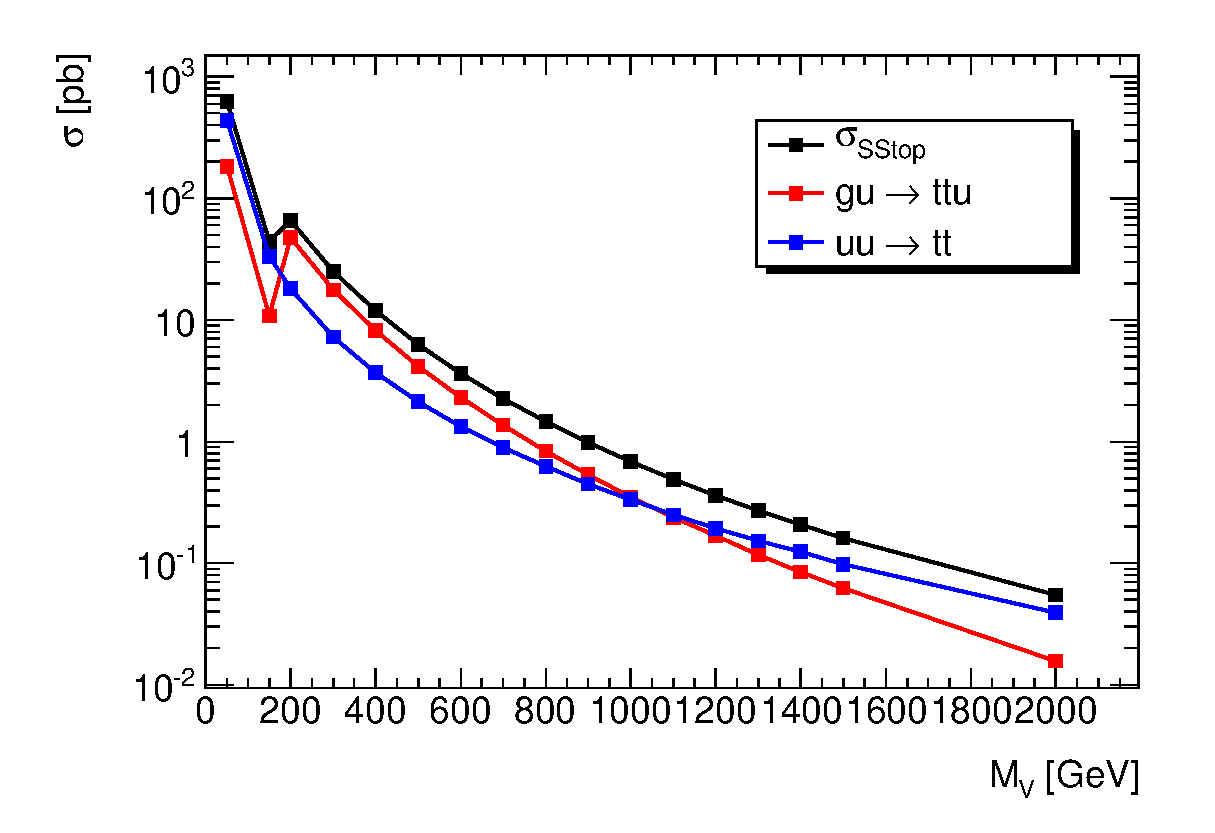
\includegraphics[width=0.6\textwidth]{appendix/appendixA/xsec_vs_mass.eps}
  \caption{
    Total cross-section of $tt\bar{u}$ (red) and $tt$ (bleue) production for different mediator mass. The total cross-section is shown in black.
  }
  \label{fig:appA:allxsec}
\end{figure}



Figure~\ref{fig:appA:fractionOftandvirtualV} shows how the various diagrams contribute to the total cross-section for the $tt+X$ final state, 
as a function of the mediator mass and for two different width. More precisely, there are two disctinct partonic 
processes: $gu \to tt\bar{u}$ ($\sigma(tt\bar{u})$) and $uu \to tt$ ($\sigma(tt)$). The total cross-section is written $\sigma(tt+X) \equiv \sigma(tt\bar{u}) + \sigma(tt)$.
The width which are considered in this section are the value calculated by MadGraph (labelled \textit{auto}) using the visible decay mode only, and a value set
by hand at $10\%$ of $m_V$.

\begin{figure}[!h!tpd]
  \centering
  \includegraphics[width=0.23\textwidth]{feyn_diags/gu_Vt_tu}     \hspace{0.5cm}
  \includegraphics[width=0.23\textwidth]{feyn_diags/gu_Vt_tu_2}   \hspace{0.8cm}
  \includegraphics[width=0.13\textwidth]{feyn_diags/other_gu_ttu} \hspace{1.0cm}
  \includegraphics[width=0.13\textwidth]{feyn_diags/uu_tt}
  \caption{
    Feynman diagram of leading order processes leading to the $tt\bar{u}$ (left) and to the $tt$ production (right), both via $V$ exchange in the $t$-channel.
  }
  \label{fig:appA:feyn_prod_ss_all}
\end{figure}

The left plot of figure~\ref{fig:appA:fractionOftandvirtualV} shows the fraction $\sigma(tt) / \sigma(tt+X)$ as a function of
$m_V$. The observed behaviour is explained by the propagator of $V$: below the $m_t$ threshold, $V$ can only be virtual and the $t$-channel has a large contribution.
At high mass, it becomes more and more difficult to produce an on-shell $V$ which makes the $t$-channel fraction larger as the mass increases. This is even
more pronounced when $\Gamma_V$ increases since it makes the probability to be virtual higher.

The right plot of figure~\ref{fig:appA:fractionOftandvirtualV} shows the impact of third diagram from figure~\ref{fig:appA:feyn_prod_ss_all} on the $tt\bar{u}$ production. 
Indeed, $V$ doesn't decay into $t\bar{u}$ in this diagram, in opposition to the diagrams describing $gu \to tV(\to t\bar{u})$. Practically, 
the fraction of $gu \to tt\bar{u}$ events with an on-shell $V$\footnote{This is defined by a Madgraph parameter $bwcut$, 
standing for Breit-Wigner Window. If $\sqrt{E_V^2 - {\vec{p}_V}^2}$ is in a window of $bwcut \times \Gamma_V$ centered to $m_V$, then $V$ is considered as on-shell. For this study, $bwcut=25$.} compared 
to all $gu \to tt\bar{u}$ events. More the $V$ width is large, more this effect is visible. The interest of this plot is to quantify the fraction of events 
which cannot be simply scaled by $\BR{V}{\chi\chi}$ for the monotop and same-sign combination (cf.~\ref{sec:comb}).

\begin{figure}[!h!tpd]
  \centering
  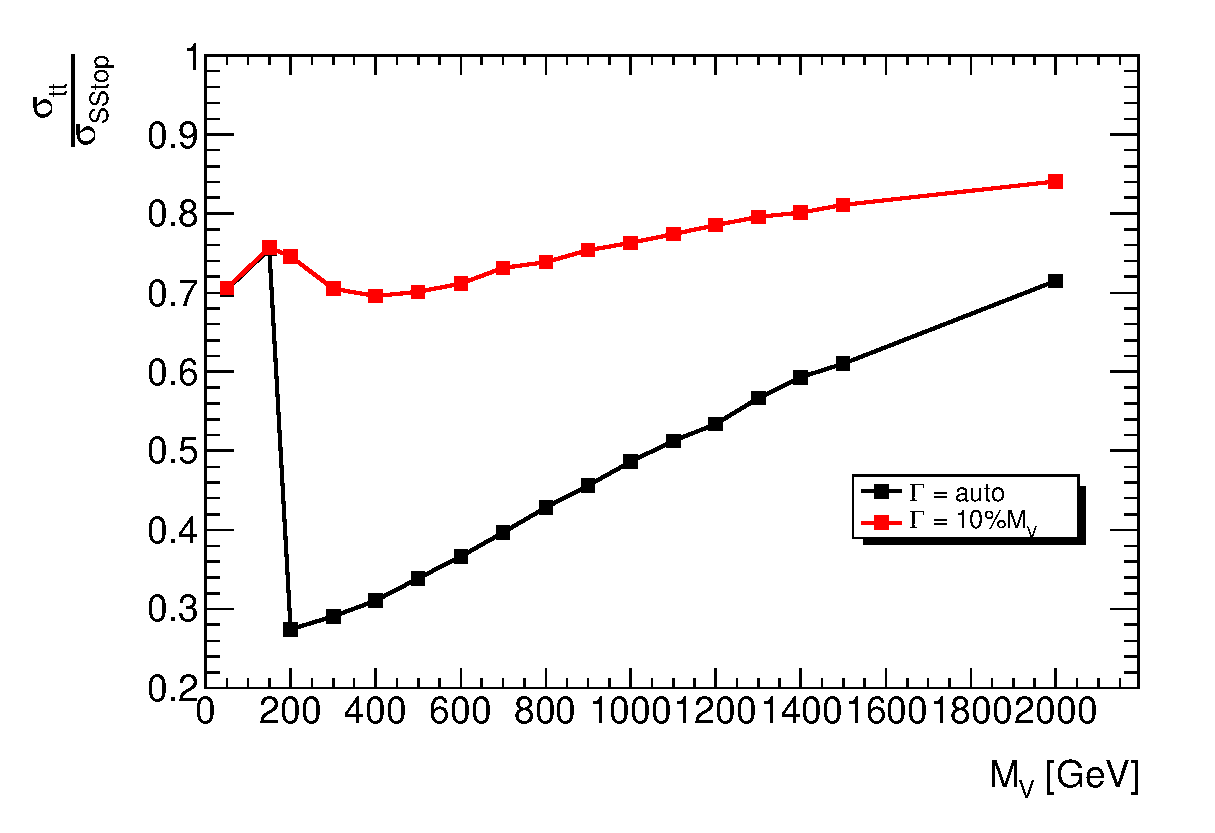
\includegraphics[width=0.48\textwidth]{appendix/appendixA/uu_tt_ratio_vs_mass.eps}
  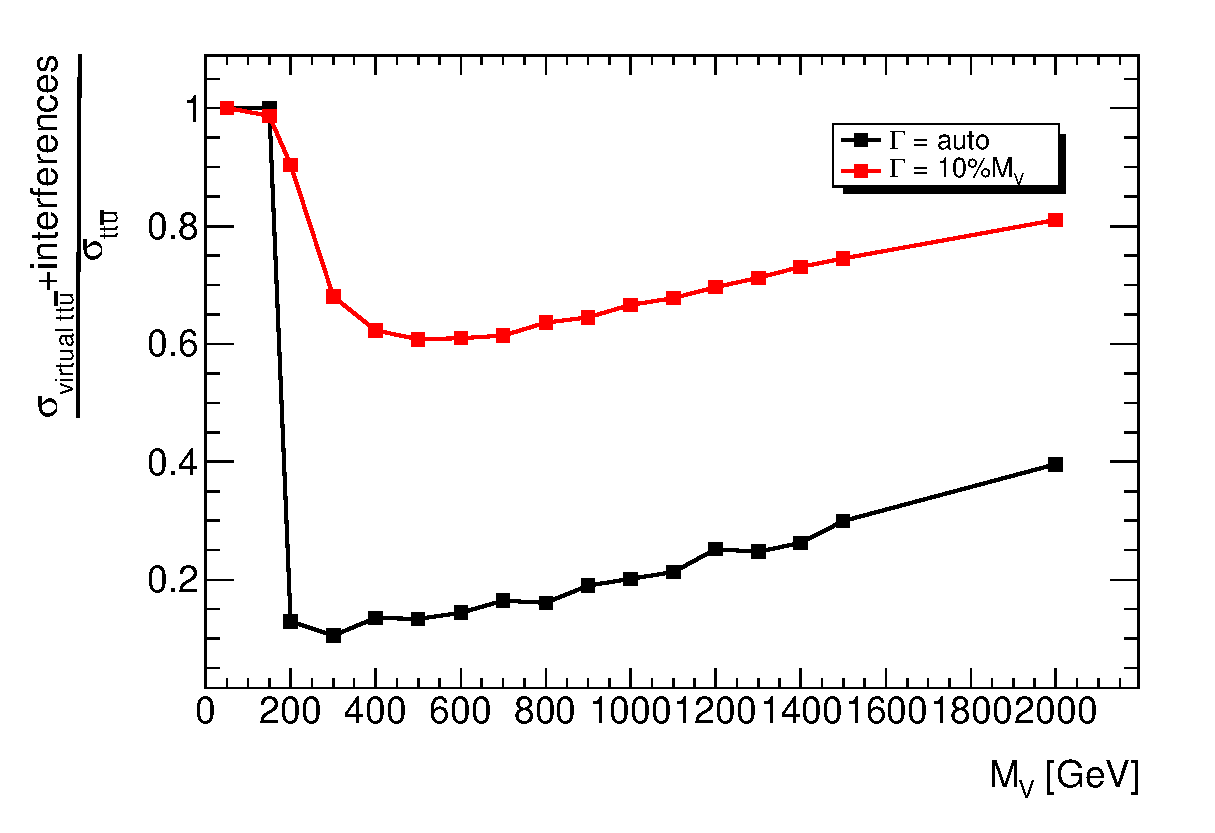
\includegraphics[width=0.48\textwidth]{appendix/appendixA/virtual_ttu_ratio_vs_mass.eps}
  \caption{
    Fraction of $t$-channel for the $tt+X$ final state as a function of the mediator mass (left) and effect of virtual $V$ contribution to 
    $gu \to tt\bar{u}$ process as a function of the mediator mass (right).
  }
  \label{fig:appA:fractionOftandvirtualV}
\end{figure}


\clearpage
\section{Mediator width effects for the non-resonant model}

\subsection{Effects on the $tV$ production}

Figure~\ref{fig:appB:pTV} and~\ref{fig:appB:pTtop} shows the $V$ mass distribution, the transverse momentum for $V$ and for the top quark coming from $V\to t\bar{u}$, for different masses and $V$ width. 
These figures are relevant independtly of the $V$ decay mode (visible or invisible). It applies then for both monotop and same-sign top final states.

\begin{figure}[!h!tpd]
  \centering
  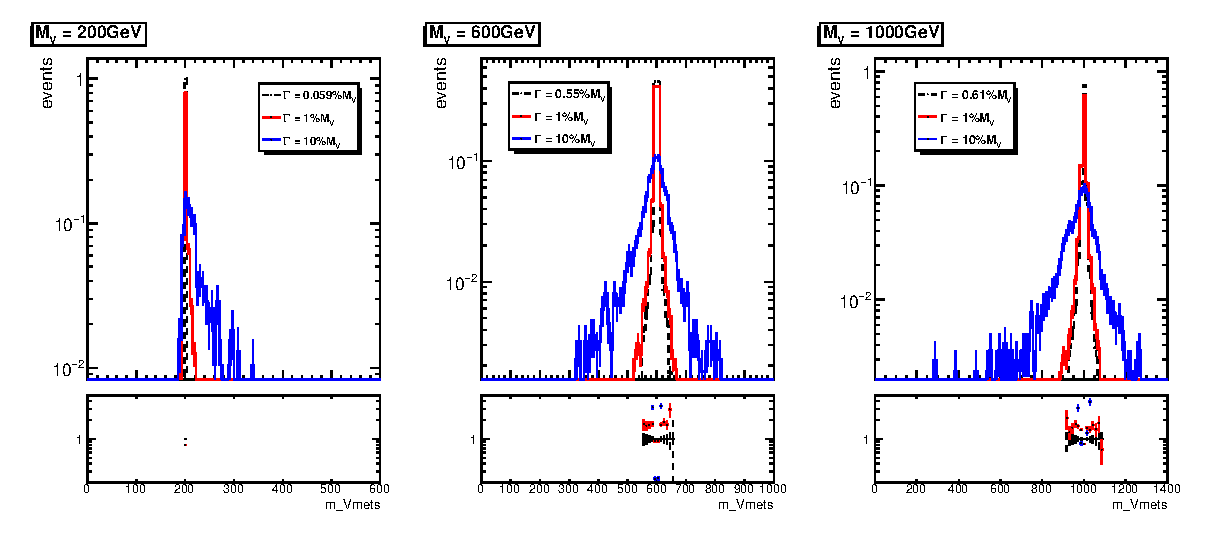
\includegraphics[width=1.0\textwidth]{appendix/appendixB/m_Vmets.eps}
  \caption{
    Distribution of $V$ invariant mass for the $gu\to tV(\to t\bar{u})$ (on-shell V) 
    for $m_V = \{200, 600, 1000\}~\GeV{}$ (from left to right) and for three different
    visible decay width (computed from Madgraph directly, $1\%$ and $10\%$).
  }   
  \label{fig:appB:Vmass}
\end{figure}


\begin{figure}[!h!tpd]
  \centering
  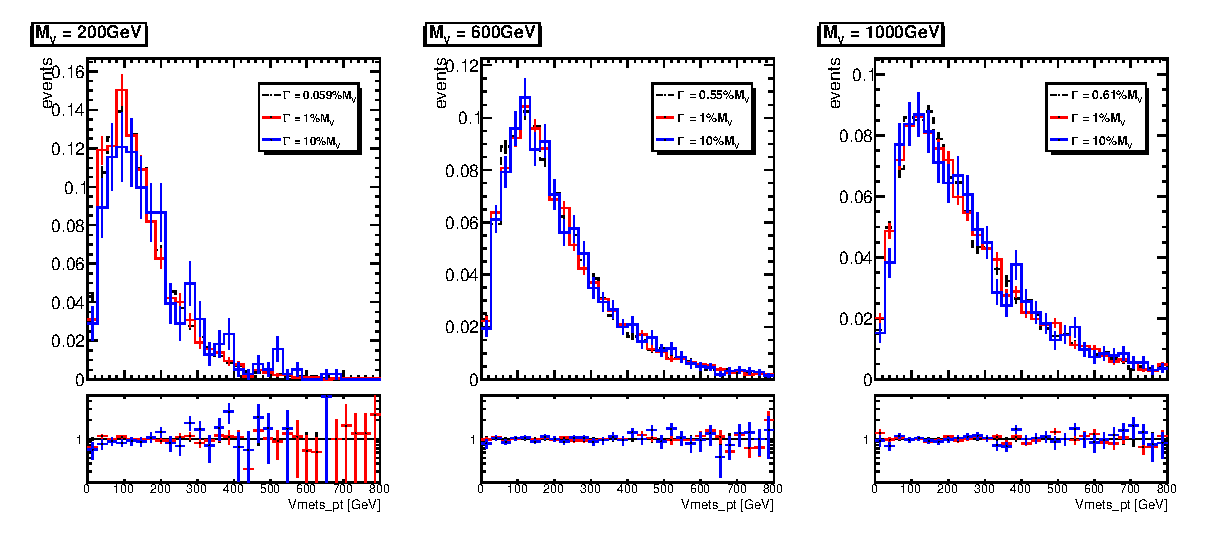
\includegraphics[width=1.0\textwidth]{appendix/appendixB/Vmets_pt.eps}
  \caption{
    Distribution of the $V$ $p_T$ for the $gu\to tV(\to t\bar{u})$ (on-shell V) for $m_V = \{200, 600, 1000\}~\GeV{}$ (from left to right) and for three different
    visible decay width (computed from Madgraph directly, $1\%$ and $10\%$).
  }
  \label{fig:appB:pTV}
\end{figure}


\begin{figure}[!h!tpd]
  \centering
  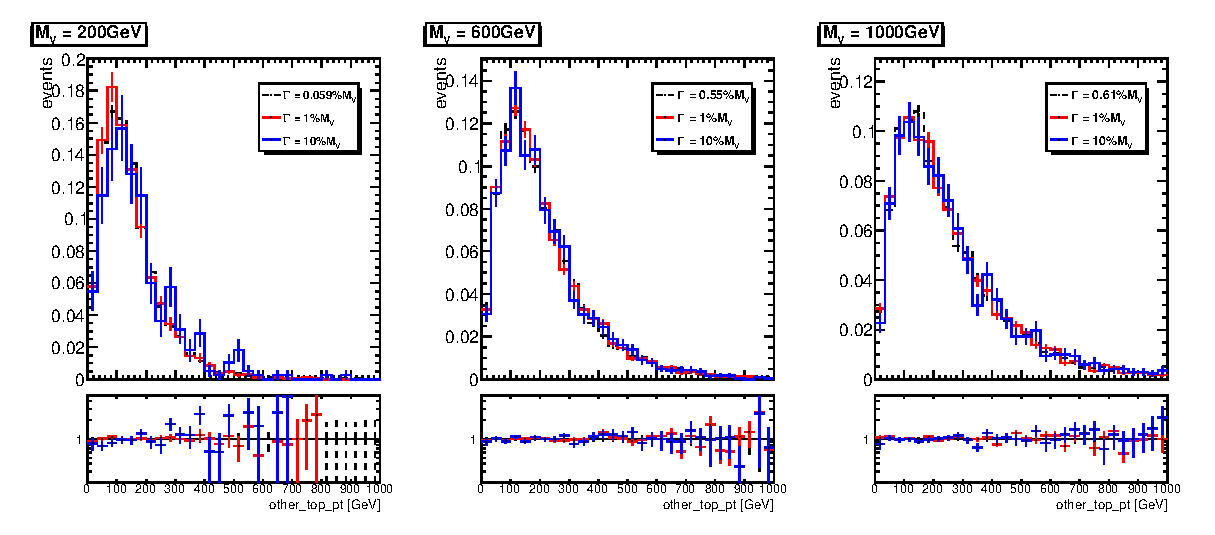
\includegraphics[width=1.0\textwidth]{appendix/appendixB/other_top_pt.eps}
  \caption{
    Distribution of the top quark $p_T$ produced in association with $V$ in $gu\to tV$ for $m_V = \{200, 600, 1000\}~\GeV{}$ (from left to right) and for three different
    visible decay width (computed from Madgraph directly, $1\%$ and $10\%$).
  }
  \label{fig:appB:pTtop}
\end{figure}



%\clearpage
\subsection{Effects on the $tt+X$ final state}
\label{sec:appB:ttXimpact}

Figures~\ref{fig:appB:pTAllTops} to~\ref{fig:appB:HT} focus on the $tt+X$ production showing the $p_T$ of all top quarks in the events, 
the leading jet $p_T$, the jet multiplicity, the $\met$, the lepton multiplicity and $H_T$. These plots
show that with $V$ width has a clear impact on some important distributions (top quark $p_T$, leading jet $p_T$, jet multiplicity, $H_T$). Section~\ref{sec:appB:tt_vs_tV} will 
demonstrate this impact is just a consequence of how the width change the relative fraction of each diagrams of Figure~\ref{fig:appA:feyn_prod_ss_all}.

\begin{figure}[!h!tpd]
  \centering
  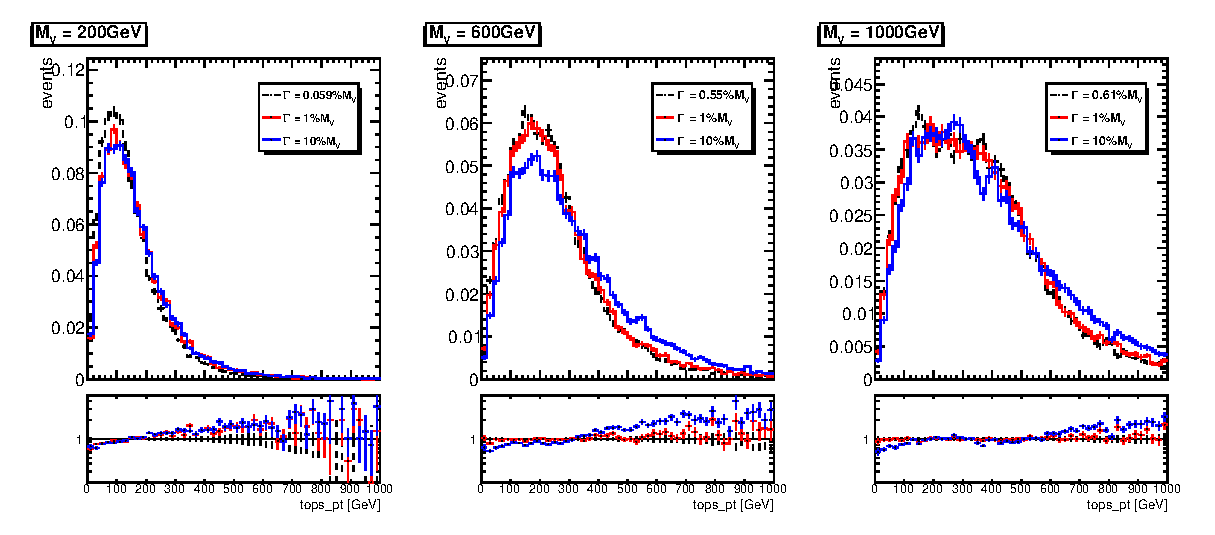
\includegraphics[width=1.0\textwidth]{appendix/appendixB/tops_pt.eps}
  \caption{
    Distribution of all top quark $p_T$ in the events for all processes leading to $tt+X$
    for $m_V = \{200, 600, 1000\}~\GeV{}$ (from left to right) and for three different
    visible decay width (computed from Madgraph directly, $1\%$ and $10\%$).
  }   
  \label{fig:appB:pTAllTops}
\end{figure}


\begin{figure}[!h!tpd]
  \centering
  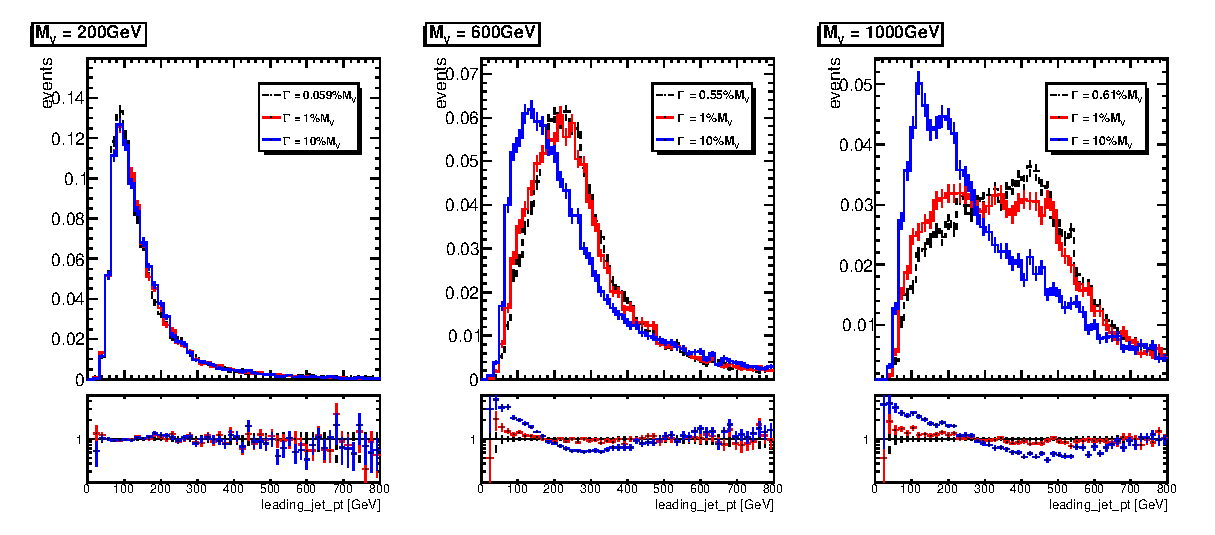
\includegraphics[width=1.0\textwidth]{appendix/appendixB/leading_jet_pt.eps}
  \caption{
      Distribution of the leading jet $p_T$ for all processes leading to $tt+X$
      for $m_V = \{200, 600, 1000\}~\GeV{}$ (from left to right) and for three different
      visible decay width (computed from Madgraph directly, $1\%$ and $10\%$).
  }   
  \label{fig:appB:Vmass}
\end{figure}


\begin{figure}[!h!tpd]
  \centering
  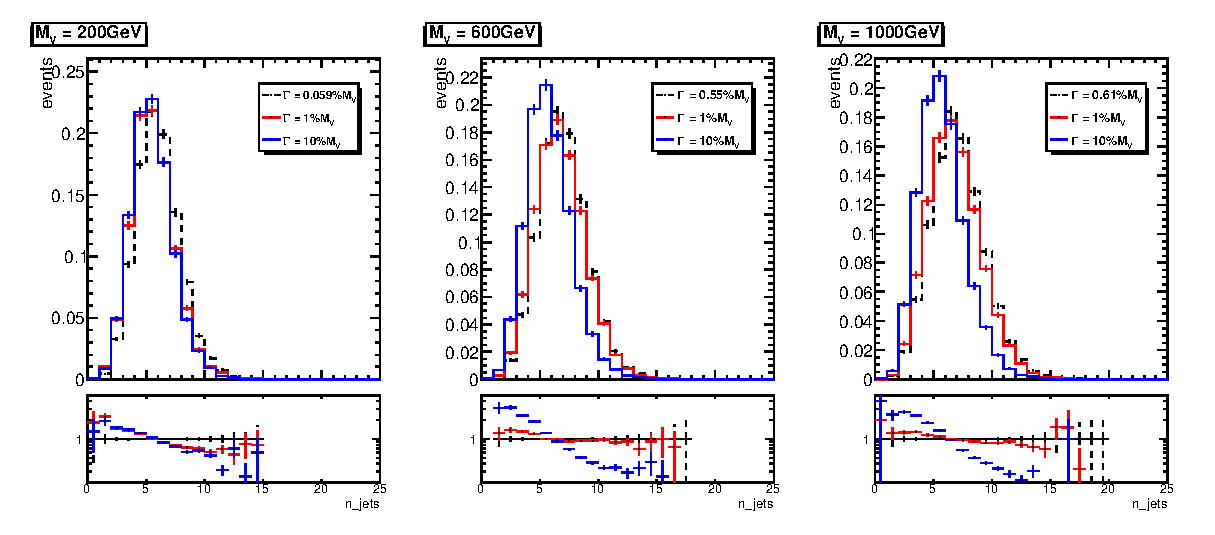
\includegraphics[width=1.0\textwidth]{appendix/appendixB/n_jets.eps}
  \caption{
      Distribution of the jet multiplicity for all processes leading to $tt+X$
      for $m_V = \{200, 600, 1000\}~\GeV{}$ (from left to right) and for three different
      visible decay width (computed from Madgraph directly, $1\%$ and $10\%$).
  }   
  \label{fig:appB:Vmass}
\end{figure}


\begin{figure}[!h!tpd]
  \centering
  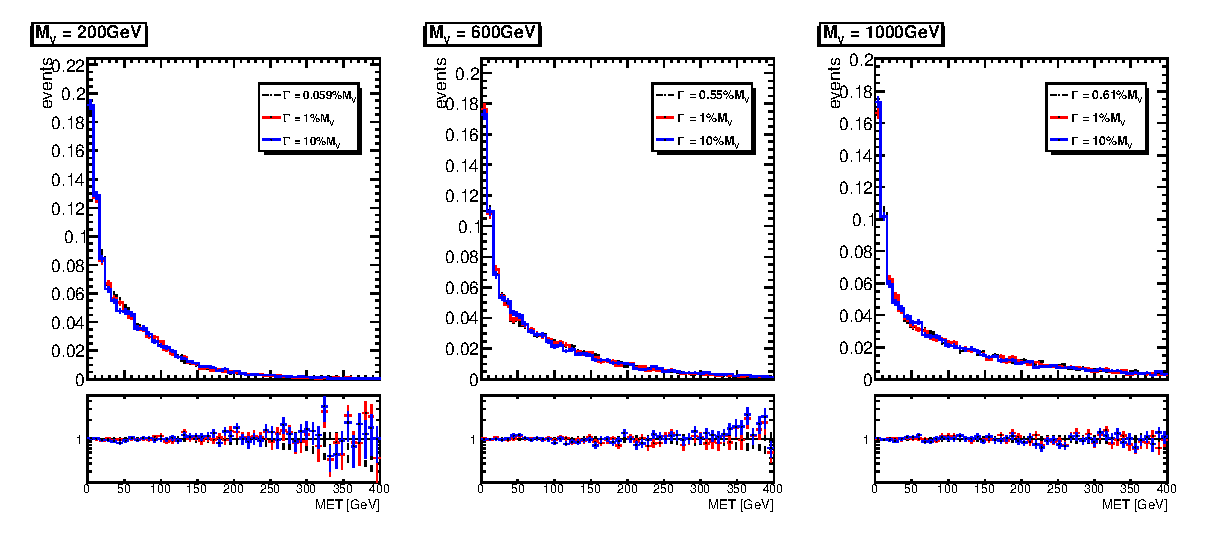
\includegraphics[width=1.0\textwidth]{appendix/appendixB/MET.eps}
  \caption{
      Distribution of the $\met$ for all processes leading to $tt+X$
      for $m_V = \{200, 600, 1000\}~\GeV{}$ (from left to right) and for three different
      visible decay width (computed from Madgraph directly, $1\%$ and $10\%$).
  }   
  \label{fig:appB:Vmass}
\end{figure}



\begin{figure}[!h!tpd]
  \centering
  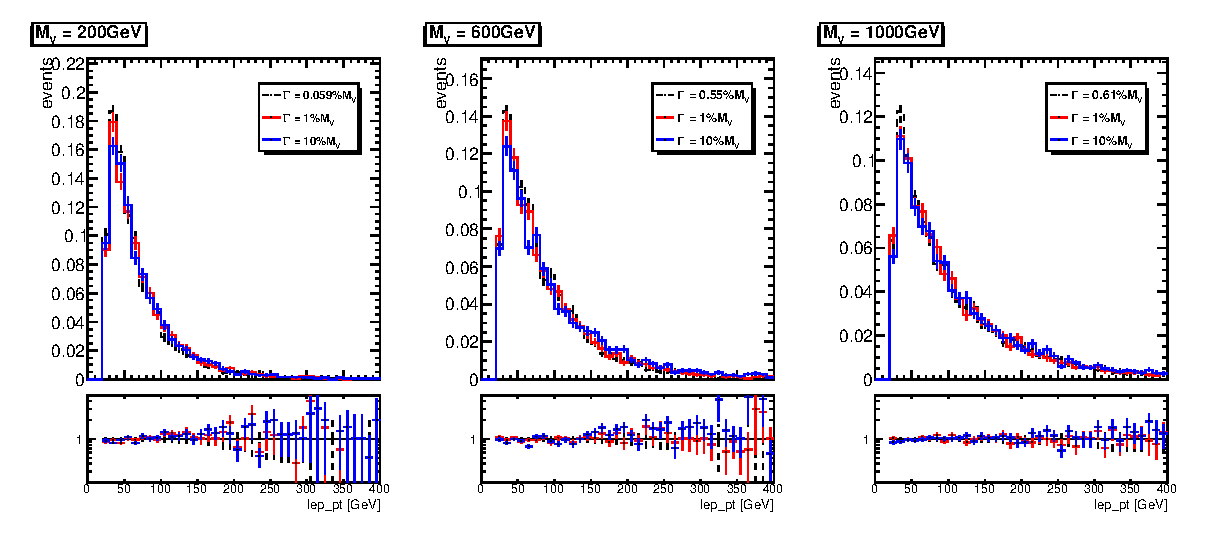
\includegraphics[width=1.0\textwidth]{appendix/appendixB/lep_pt.eps}
  \caption{
      Distribution of the lepton $p_T$ for all processes leading to $tt+X$
      for $m_V = \{200, 600, 1000\}~\GeV{}$ (from left to right) and for three different
      visible decay width (computed from Madgraph directly, $1\%$ and $10\%$).
  }   
  \label{fig:appB:Vmass}
\end{figure}


\begin{figure}[!h!tpd]
  \centering
  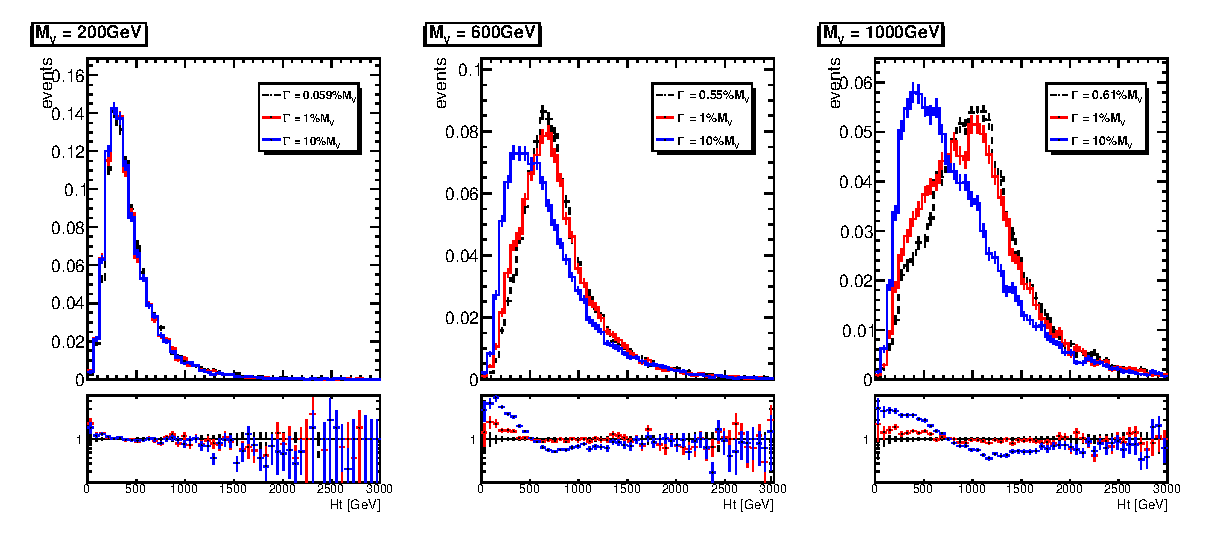
\includegraphics[width=1.0\textwidth]{appendix/appendixB/Ht.eps}
  \caption{
      Distribution of the $p_T$ scalar sum ($H_T$) for all processes leading to $tt+X$
      for $m_V = \{200, 600, 1000\}~\GeV{}$ (from left to right) and for three different
      visible decay width (computed from Madgraph directly, $1\%$ and $10\%$).
  }   
  \label{fig:appB:HT}
\end{figure}


\clearpage
\subsection{Comparison of $gu \to tV(\to t\bar{u})$ and $uu\to tt$ processes}
\label{sec:appB:tt_vs_tV}

Figures~\ref{fig:appB:pTAllTops_stchannel} to~\ref{fig:appB:HT_stchannel} show the width effect on top $p_T$, leading jet $p_T$, jet multiplicity and $H_T$, 
separately for $gu \to tV(\to t\bar{u})$ and $uu \to tt$ processes. These plot show the important kinematic differences between the $tt$ production 
via a $t$-channel exchange of the mediator and the direct production of the mediator, decaying into $t\bar{u}$. On each of these process, the width doesn't
change at all the kinematics but it does change the relative importance of each process, as shown in section~\ref{sec:appA}. This explains then the
width impact observed in section~\ref{sec:appB:ttXimpact}.


\begin{figure}[!h!tpd]
  \centering
  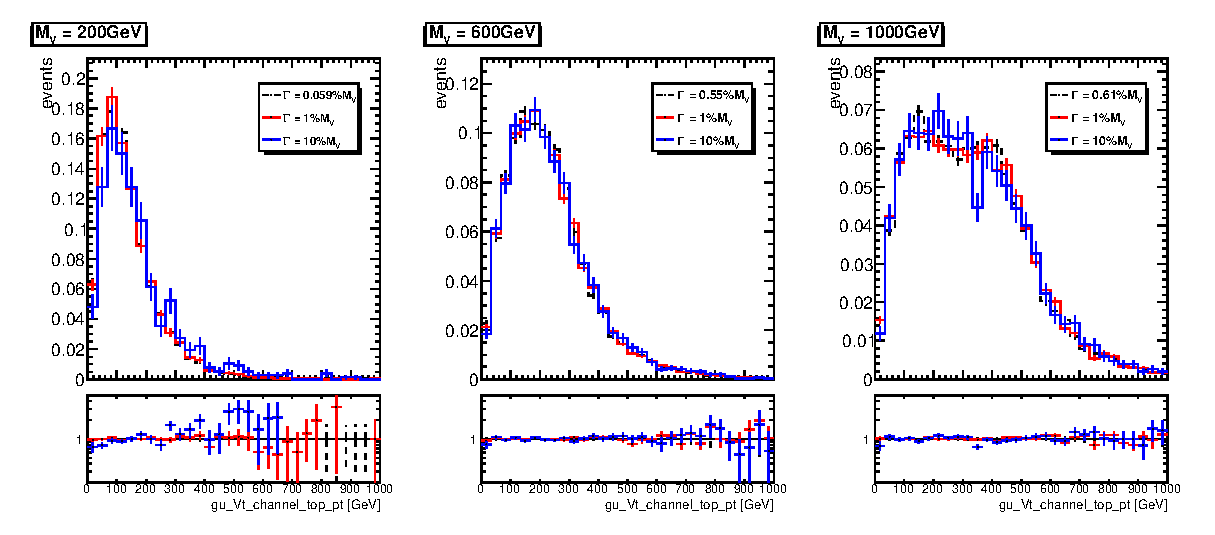
\includegraphics[width=1.0\textwidth]{appendix/appendixB/gu_Vt_channel_top_pt.eps} \\
  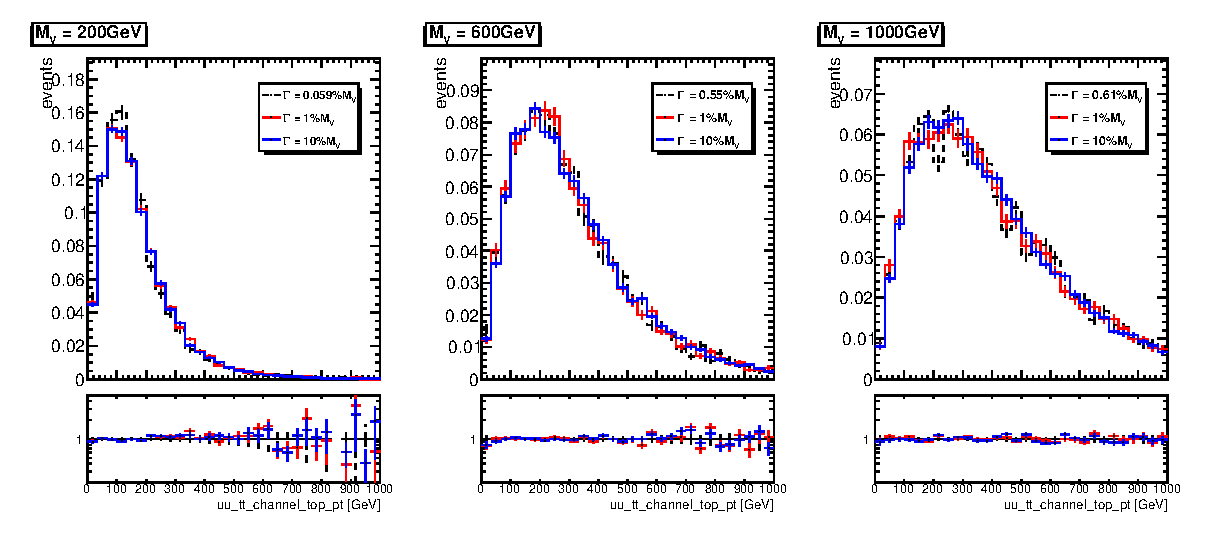
\includegraphics[width=1.0\textwidth]{appendix/appendixB/uu_tt_channel_top_pt.eps}
  \caption{
      Distribution of all top quark $p_T$ in the events for all processes leading to $tt+X$
      for $m_V = \{200, 600, 1000\}~\GeV{}$ (from left to right) and for three different
      visible decay width (computed from Madgraph directly, $1\%$ and $10\%$). Top plots show $gu \to tt \bar{u}$ and bottom plots show $uu \to tt$.
  }   
  \label{fig:appB:pTAllTops_stchannel}
\end{figure}


\begin{figure}[!h!tpd]
  \centering
  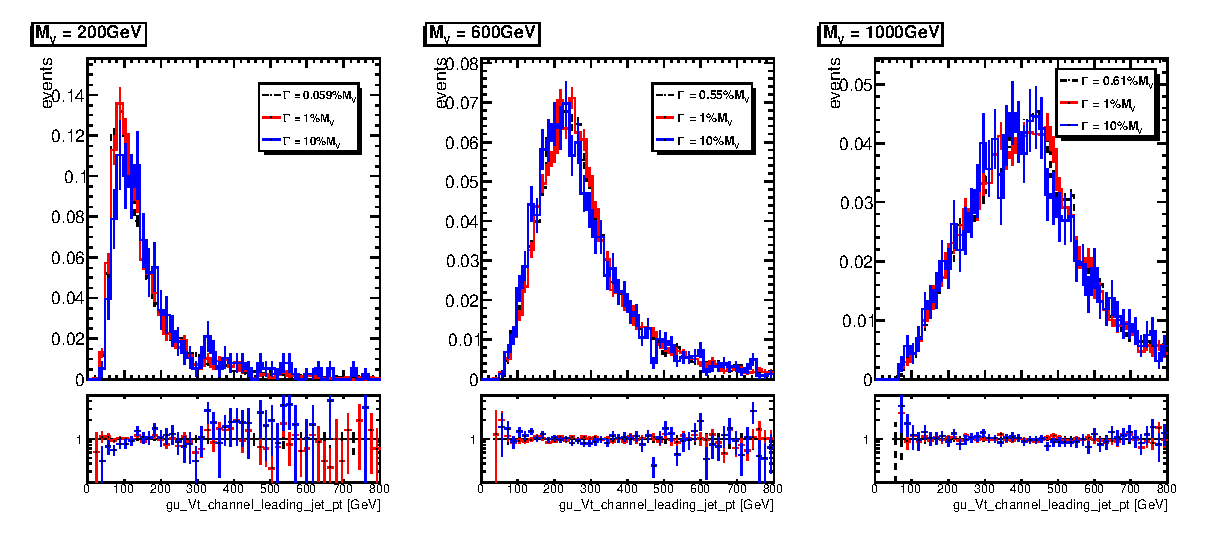
\includegraphics[width=1.0\textwidth]{appendix/appendixB/gu_Vt_channel_leading_jet_pt.eps}\\
  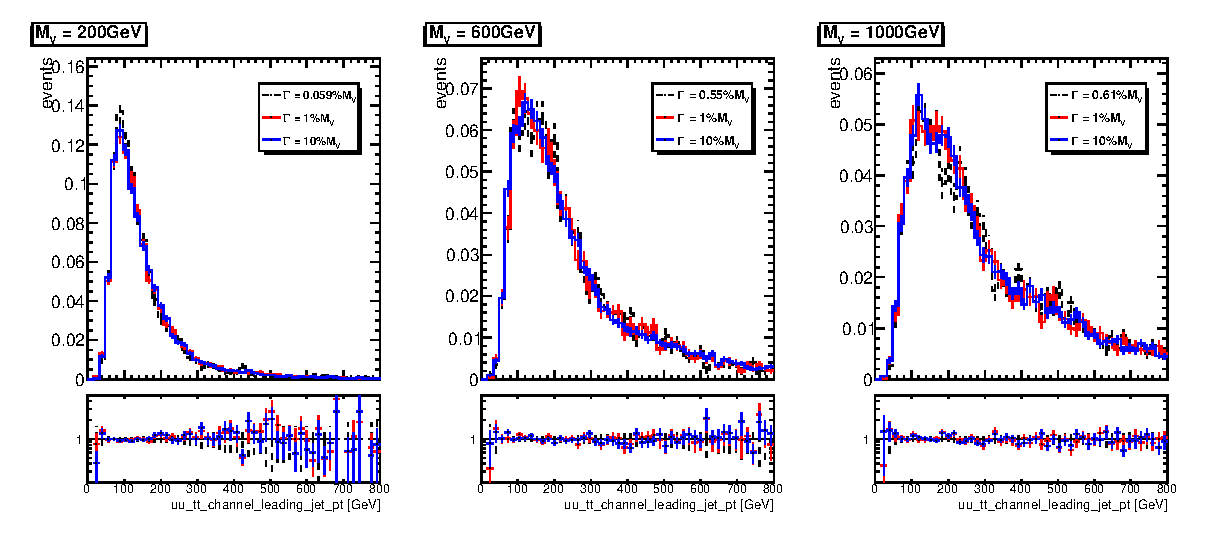
\includegraphics[width=1.0\textwidth]{appendix/appendixB/uu_tt_channel_leading_jet_pt.eps}
  \caption{
      Distribution of the leading jet $p_T$ for all processes leading to $tt+X$
      for $m_V = \{200, 600, 1000\}~\GeV{}$ (from left to right) and for three different
      visible decay width (computed from Madgraph directly, $1\%$ and $10\%$). Top plots show $gu \to tt \bar{u}$ and bottom plots show $uu \to tt$.
  }   
  \label{fig:appB:Vmass}
\end{figure}


\begin{figure}[!h!tpd]
  \centering
  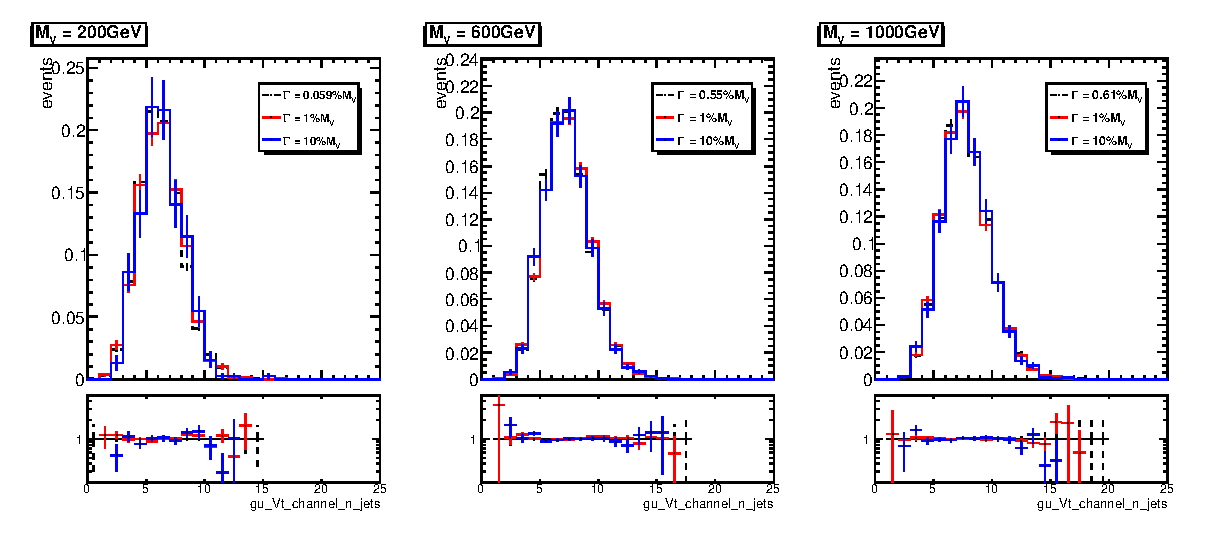
\includegraphics[width=1.0\textwidth]{appendix/appendixB/gu_Vt_channel_n_jets.eps}\\
  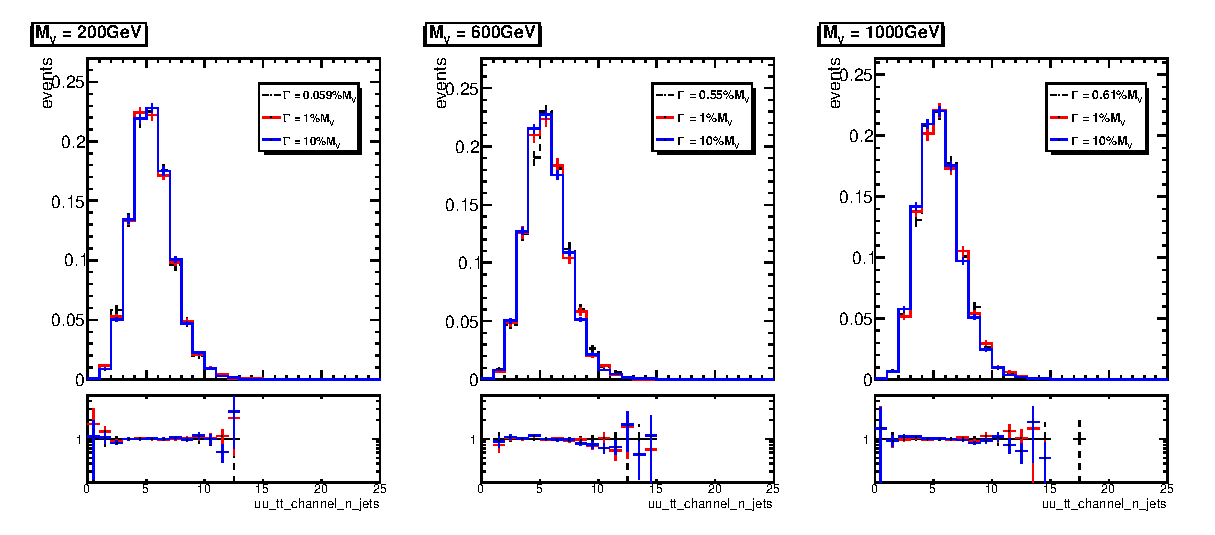
\includegraphics[width=1.0\textwidth]{appendix/appendixB/uu_tt_channel_n_jets.eps}
  \caption{
      Distribution of the jet multiplicity for all processes leading to $tt+X$
      for $m_V = \{200, 600, 1000\}~\GeV{}$ (from left to right) and for three different
      visible decay width (computed from Madgraph directly, $1\%$ and $10\%$). Top plots show $gu \to tt \bar{u}$ and bottom plots show $uu \to tt$.
  }   
  \label{fig:appB:Vmass}
\end{figure}

\begin{figure}[!h!tpd]
  \centering
  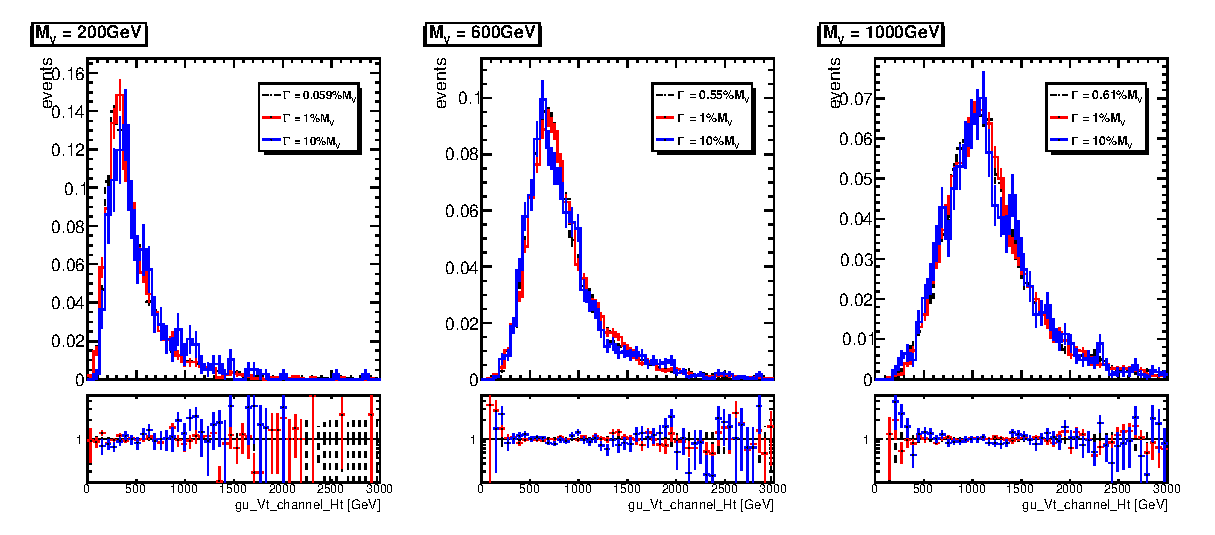
\includegraphics[width=1.0\textwidth]{appendix/appendixB/gu_Vt_channel_Ht.eps}\\
  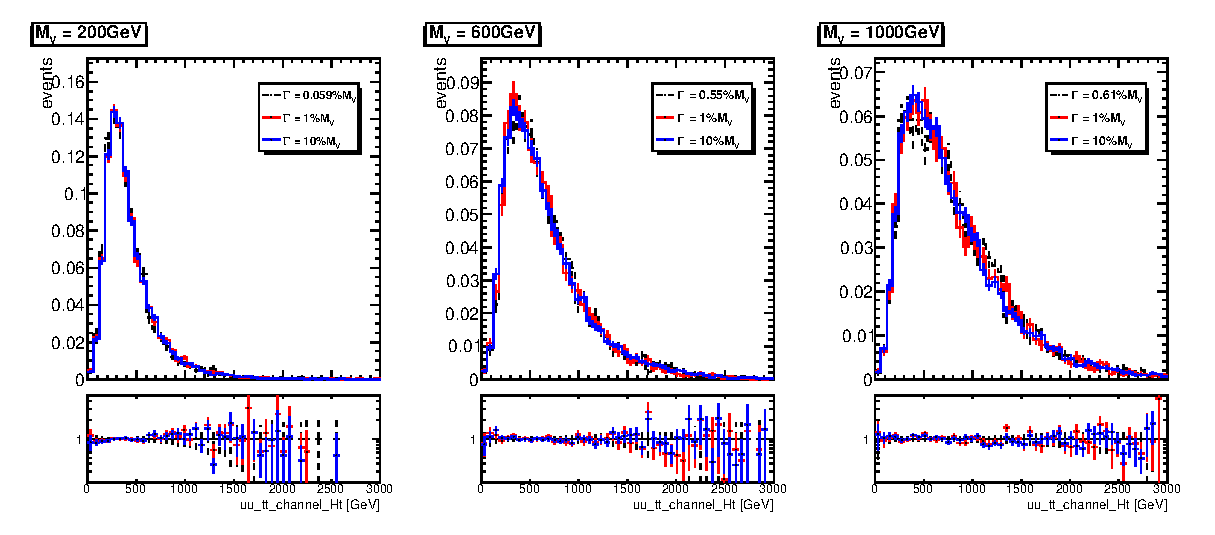
\includegraphics[width=1.0\textwidth]{appendix/appendixB/uu_tt_channel_Ht.eps}
  \caption{
    Distribution of the $p_T$ scalar sum ($H_T$) for all processes leading to $tt+X$
    for $m_V = \{200, 600, 1000\}~\GeV{}$ (from left to right) and for three different
    visible decay width (computed from Madgraph directly, $1\%$ and $10\%$). Top plots show $gu \to tt \bar{u}$ and bottom plots show $uu \to tt$.
  }   
  \label{fig:appB:HT_stchannel}
\end{figure}



\clearpage
\section{Signal and background distributions ($tt+X$ final state)}

In this section, the shape of some key distributions are compared for for the two signal processes, namely $gu \to tt \bar{u}$ and $uu \to tt$, 
and the two main backgrounds relevant for the $tt+X$ final state, namely $t\bar{t}$ (via charge mis-reconstruction) and $t\bar{t} + V$. The 
distributions are obtained at the truth hadronic level, without any detector effects. The objects are selected using criteria close from those
used in the Run 1 analysis.


\begin{figure}[!h!tpd]
  \centering
  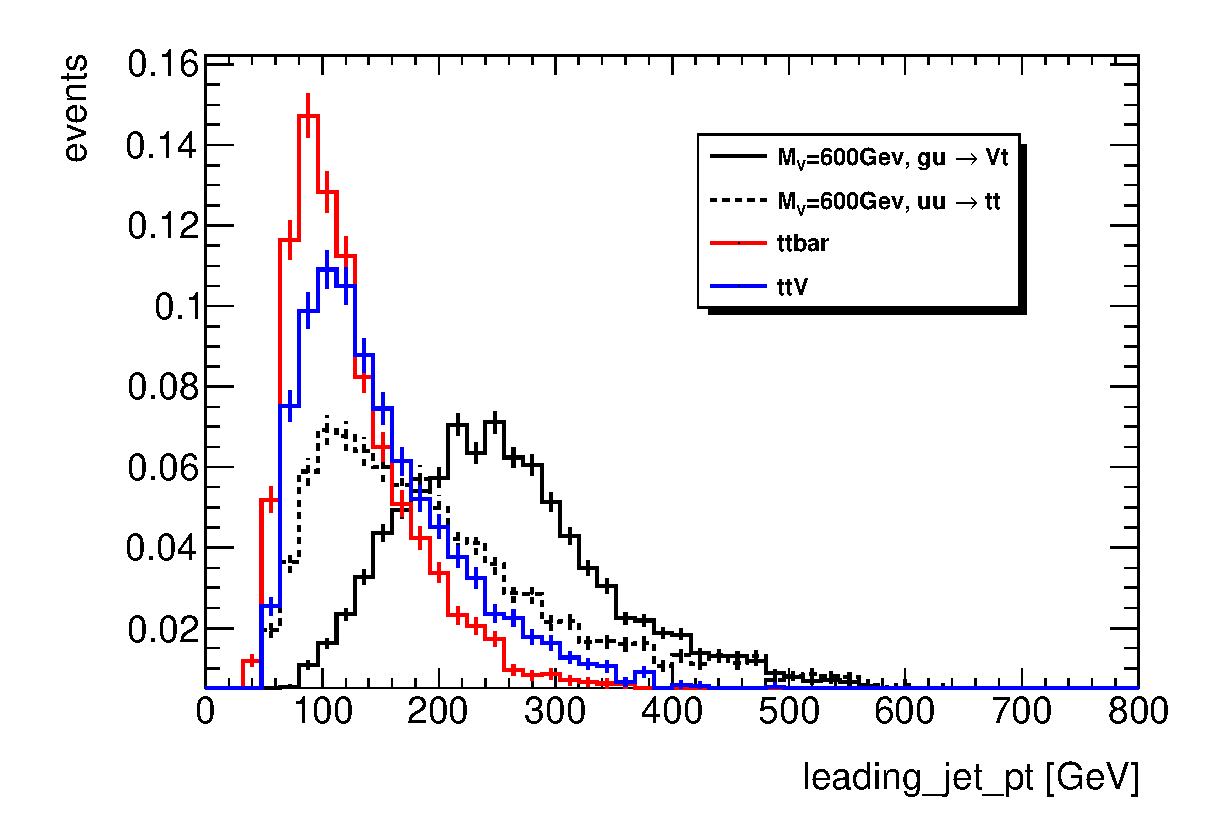
\includegraphics[width=0.48\textwidth]{appendix/appendixC/leading_jet_pt.eps}
  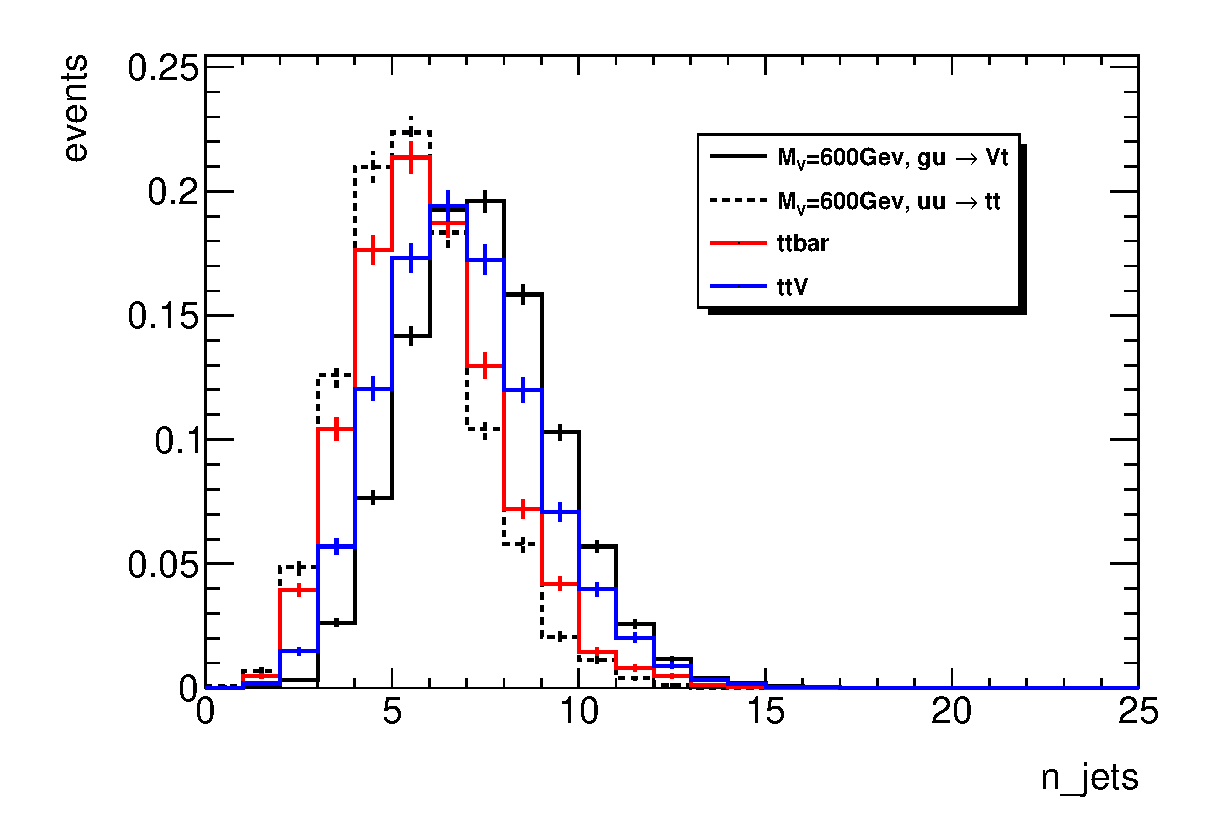
\includegraphics[width=0.48\textwidth]{appendix/appendixC/n_jets.eps}
  \caption{
      Distribution of the leading jet $p_T$ for signals ($m_V=600~\GeV{}$, $\Gamma_V$ computed in MadGraph) and backgrounds at the (hadronic) thruth level.
  }   
  \label{fig:appB:Vmass}
\end{figure}


%\begin{figure}[!h!tpd]
%  \centering
%  \caption{
%      Distribution of the jet multiplicity for all processes leading to $tt+X$
%      for $m_V = \{200, 600, 1000\}~\GeV{}$ (from left to right) and for three different
%      visible decay width (computed from Madgraph directly, $1\%$ and $10\%$).
%  }   
%  \label{fig:appB:Vmass}
%\end{figure}


\begin{figure}[!h!tpd]
  \centering
  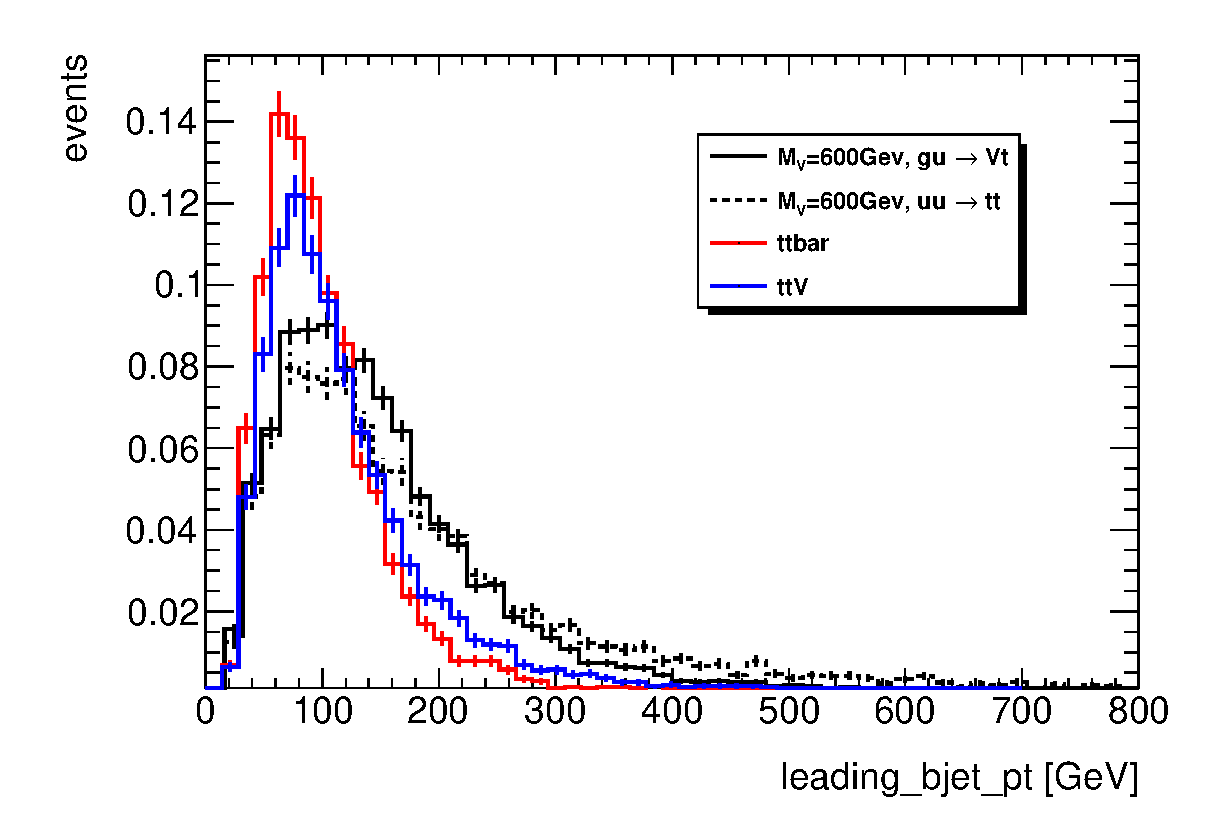
\includegraphics[width=0.48\textwidth]{appendix/appendixC/leading_bjet_pt.eps}
  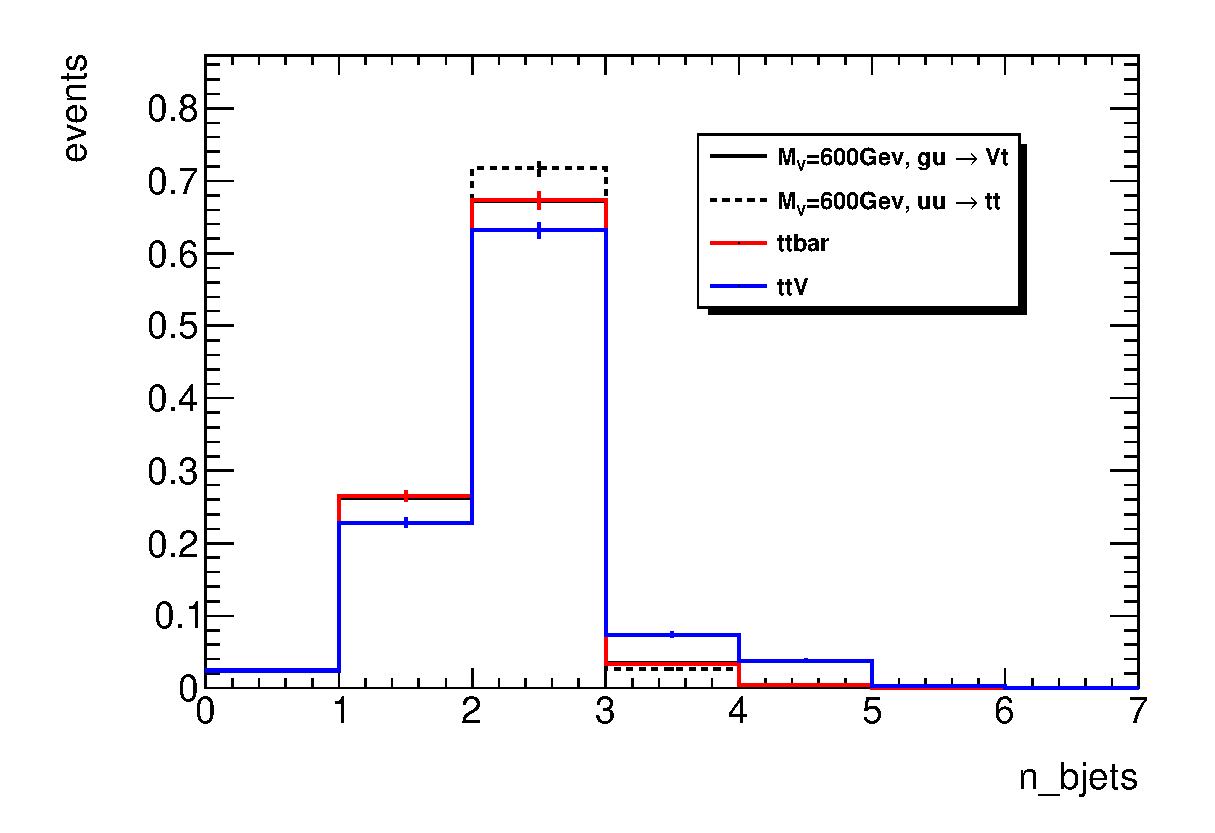
\includegraphics[width=0.48\textwidth]{appendix/appendixC/n_bjets.eps}
  \caption{
      Distribution of the leading jet $p_T$ for signals ($m_V=600~\GeV{}$, $\Gamma_V$ computed in MadGraph) and backgrounds at the (hadronic) thruth level.
  }   
  \label{fig:appB:Vmass}
\end{figure}


%\begin{figure}[!h!tpd]
%  \centering
%
%  \caption{
%      Distribution of the jet multiplicity for all processes leading to $tt+X$
%      for $m_V = \{200, 600, 1000\}~\GeV{}$ (from left to right) and for three different
%      visible decay width (computed from Madgraph directly, $1\%$ and $10\%$).
%  }   
%  \label{fig:appB:Vmass}
%\end{figure}


\begin{figure}[!h!tpd]
  \centering
  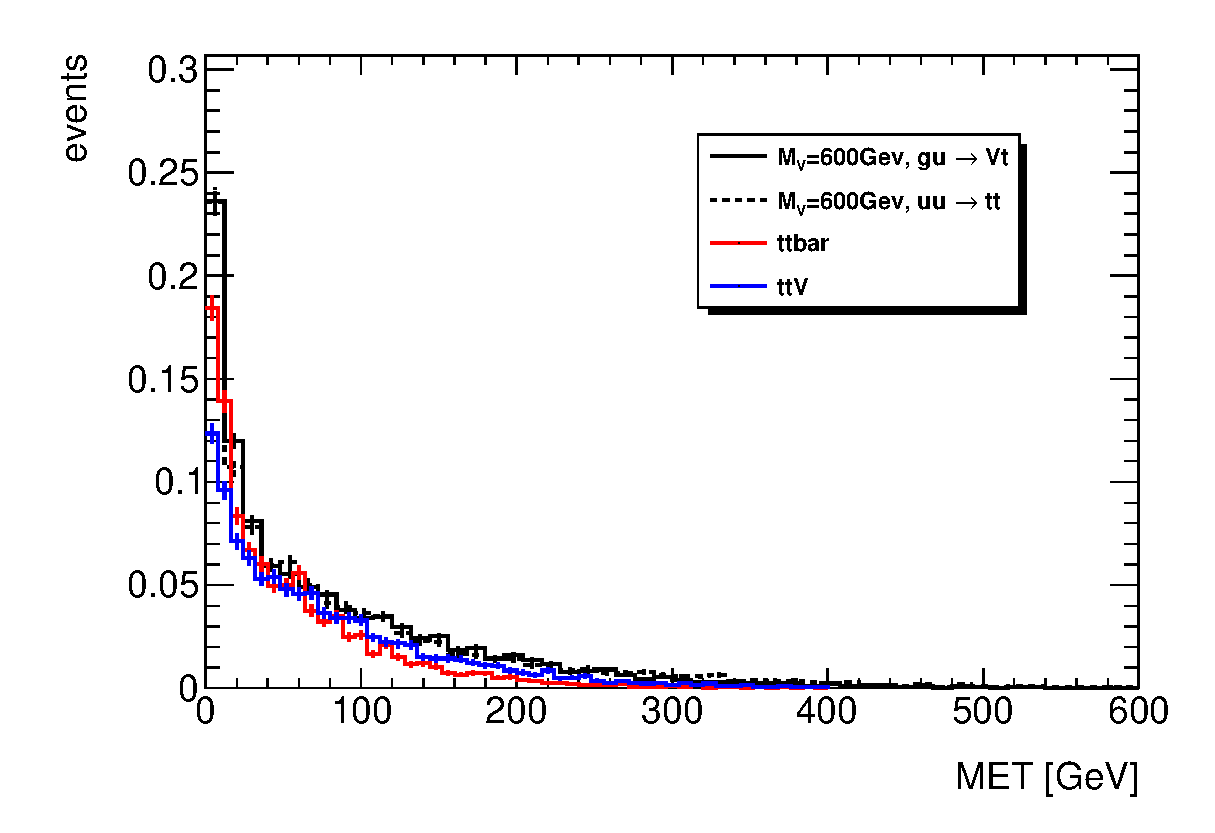
\includegraphics[width=0.48\textwidth]{appendix/appendixC/MET.eps}
  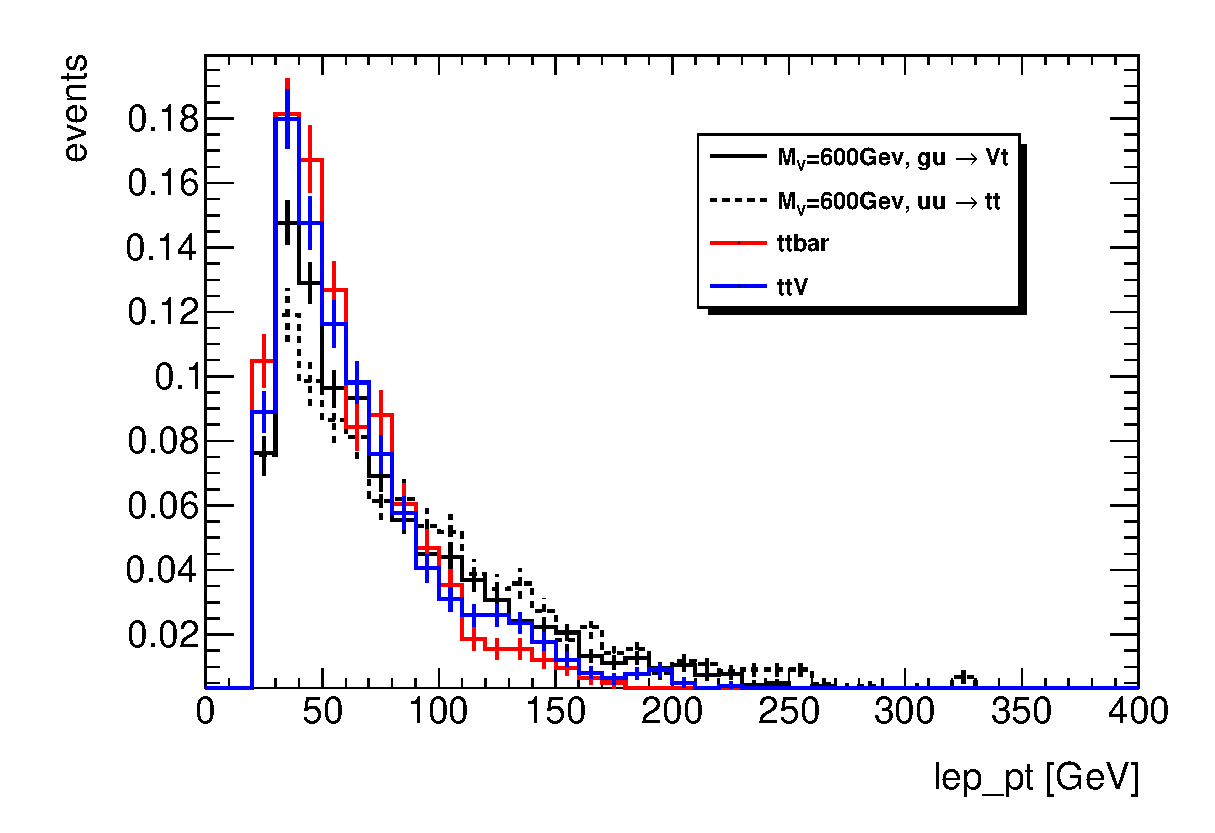
\includegraphics[width=0.48\textwidth]{appendix/appendixC/lep_pt.eps} 
 \caption{
      Distribution of the $\met$ for signals ($m_V=600~\GeV{}$, $\Gamma_V$ computed in MadGraph) and backgrounds at the (hadronic) thruth level.
  }   
  \label{fig:appB:Vmass}
\end{figure}

%\begin{figure}[!h!tpd]
%  \centering
% 
%  \caption{
%      Distribution of the lepton $p_T$ for all processes leading to $tt+X$
%      for $m_V = \{200, 600, 1000\}~\GeV{}$ (from left to right) and for three different
%      visible decay width (computed from Madgraph directly, $1\%$ and $10\%$).
%  }   
%  \label{fig:appB:Vmass}
%\end{figure}


\begin{figure}[!h!tpd]
  \centering
  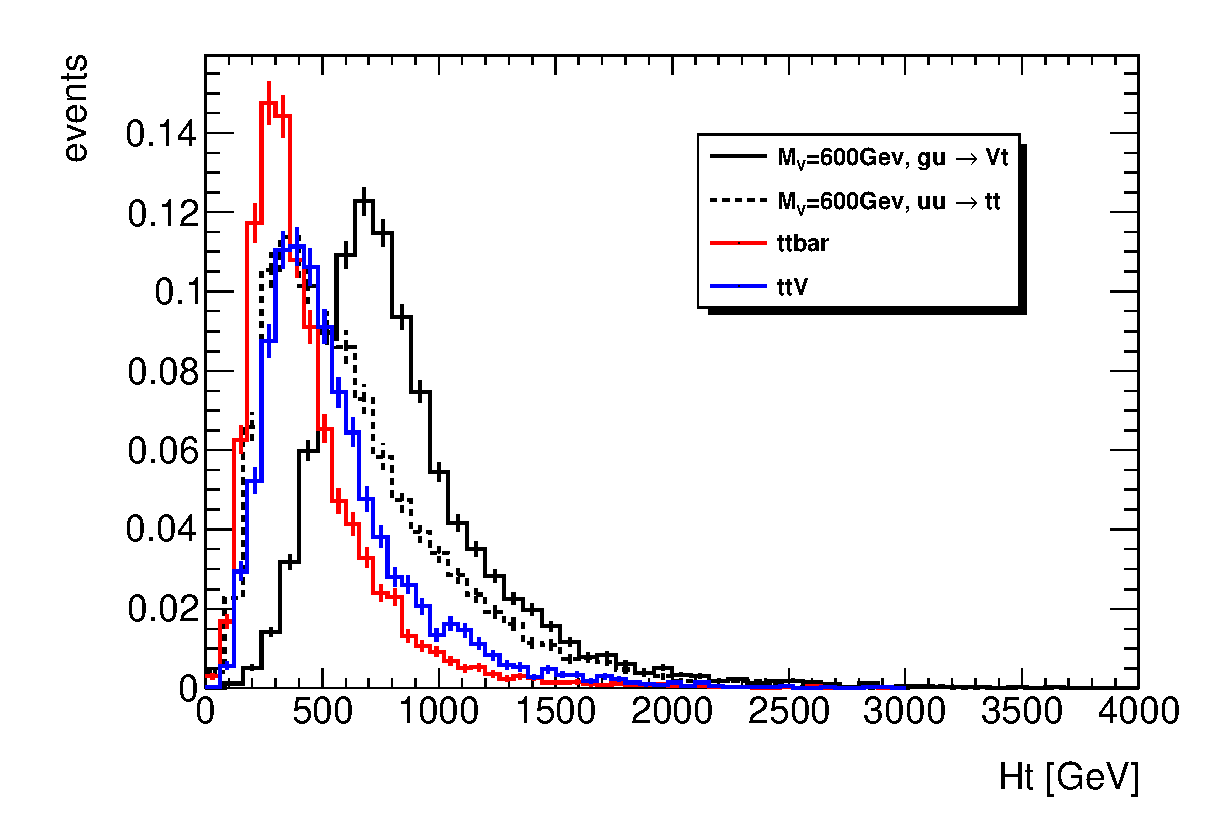
\includegraphics[width=0.65\textwidth]{appendix/appendixC/Ht.eps}
  \caption{
      Distribution of the $p_T$ scalar sum ($H_T$) for signals ($m_V=600~\GeV{}$, $\Gamma_V$ computed in MadGraph) and backgrounds at the (hadronic) thruth level.
  }   
  \label{fig:appB:HT}
\end{figure}




\end{document}
